\documentclass[twocolumn]{mnras}

% Paper packages
\usepackage{graphicx}
\usepackage{amsmath}
\usepackage{amssymb}
\usepackage{booktabs}

% Define astronomical units
\newcommand{\msun}{\ensuremath{M_{\odot}}}
\newcommand{\pc}{\ensuremath{\rm pc}}
\newcommand{\kms}{\ensuremath{\rm km\,s^{-1}}}

\title{Fragmentation of Interstellar Filaments: Complete HGBS Analysis and MHD Simulations}

\author[G.~J.~White]{G.~J.~White$^{1,2}$\\
$^{1}$School of Physical Sciences, The Open University, Walton Hall, Milton Keynes, MK7 6AA, UK\\
$^{2}$Rutherford Appleton Laboratory, Harwell Science and Innovation Campus, Didcot, OX11 0QX, UK}

\begin{document}

\maketitle

\begin{abstract}
We present a complete HGBS analysis of filament core spacing, combined with 2,860 self-gravitating MHD simulations testing whether observed spacings follow the classical $4\times$ prediction.

\textbf{Observational results with critical limitations}. Pairwise median statistics give $\lambda/W \approx 2.8$ across 8 HGBS regions with Gaia DR3 distances, but for large filaments (Orion B: $N = 1,844$ cores) this statistic converges to $L/3$ and may measure overall filament scale rather than true fragmentation wavelength. Published nearest-neighbour analyses report $\lambda/W \approx 2.0$--$2.2$ (different methodologies, not computed here). The 3D-corrected pairwise median ($\lambda/W \approx 3.3$--$3.9$) encompasses the classical $4\times$ prediction within uncertainties. Which statistic measures true fragmentation wavelength requires HGBS skeleton data for proper nearest-neighbour analysis.

\textbf{Primary theoretical conclusion: RTC null result}. The Realistic Turbulence Campaign (1,200 simulations with physical ISM turbulence, Mach 2--4, free boundaries) produces \textbf{zero} simulations within the HGBS observational window. All RTC results give $\lambda/W \geq 3.75$ (mean 10.8, median 7.3). This demonstrates that ideal isothermal MHD cannot reproduce HGBS core spacings under realistic free-boundary conditions.

\textbf{Critical theoretical limitation: Extrapolation gap}. The calibration $\lambda_{\rm frag} = (1.11 \pm 0.12)\lambda_{\rm MJ}$ comes from near-critical simulations ($f \approx 1.0$--$1.2$) where $\lambda/W$ is measurable. HGBS filaments have $f \approx 1.5$--$3.0$, where radial collapse prevents direct $\lambda/W$ measurement. This $\pm$20--30\% extrapolation uncertainty dominates the systematic error budget.

\textbf{Radial confinement constraint}. The absence of observational signatures for radial confinement in HGBS filaments (velocity profiles, external pressure, aspect ratios) suggests that free-boundary conditions better represent real filaments than artificial rigid walls. The RTC null result (0/1,200 matches) should therefore be weighted more heavily than rigid cylinder results (9/45 matches with reflecting walls).

\textbf{Field geometry crisis}. Perpendicular-field simulations predict $\lambda/W \approx 1.25$ (or $\approx 2.02$ after width normalisation), below both nearest-neighbour observations ($\approx 2.0$--$2.2$) and pairwise median ($\approx 2.8$). Since $\sim$90\% of filaments are perpendicular to the mean field (Planck 2016), this creates an independent theoretical crisis: the dominant filament population should produce shorter spacings than observed.

\textbf{Implications}. Resolving whether filaments fragment at the classical $4\times$ scale requires: (1) proper nearest-neighbour analysis with HGBS skeleton data; (2) field geometry measurements at fragmentation scales; (3) observational constraints on radial confinement; (4) bridging the extrapolation gap ($f \approx 1.2$--$1.5$).
\end{abstract}

\begin{keywords}
stars: formation -- ISM: structure -- ISM: filaments -- MHD -- turbulence
\end{keywords}


\section{INTRODUCTION}

The \textit{Herschel} Space Observatory established that filaments are the fundamental structures within which star formation occurs in molecular clouds \citep{Andre2010}. Two key observational results emerged: (1) a characteristic filament width of $\sim$0.1 pc across diverse environments \citep{Arzoumanian2011}, and (2) a critical mass-per-unit-length of $M_{\rm line,crit} \approx 16~M_\odot$/pc \citep{Ostriker1964}.

Classical fragmentation theory \citep{Inutsuka1992} predicts that isothermal gas cylinders fragment at a wavelength of approximately $4\times$ the filament width. For the characteristic HGBS filament width of $0.10$ pc, this predicts a core spacing of $\sim0.4$ pc. Original HGBS analyses measured core spacings of $\sim0.2$ pc—nearly a factor of two smaller than the theoretical prediction. However, with the adoption of Gaia DR3-based distances \citep{Zhang2023}, the measured spacings have increased to $\sim0.28$ pc, reducing the discrepancy with theory to a factor of 1.4.

Two primary explanations have been proposed for this discrepancy. First, \textbf{hierarchical fragmentation}: high-resolution studies revealed that filaments consist of velocity-coherent fibers \citep{Hacar2013}, and recent work in Orion B \citep{Yang2024} showed that while filament-to-core spacing is $\sim2$--$3\times$, fiber-to-core spacing recovers the classical $4\times$ prediction. This suggests the apparent sub-Jeans spacing at the filament level may reflect projection/averaging effects from measuring across hierarchical structures rather than a true modified fragmentation wavelength.

Second, \textbf{magnetic tension}: longitudinal magnetic fields resist bending during fragmentation, preferentially stabilising long-wavelength perturbations and shifting the most unstable mode to shorter wavelengths \citep{Nakamura1993}. For equipartition-strength fields ($\beta \sim 1$--$3$), this mechanism predicts $\lambda/W \approx 2.4$--$3.2$, overlapping with HGBS observations.

In this paper, we present the first complete HGBS analysis across all 8 high-confidence regions, combined with self-gravitating MHD simulations to test these competing explanations.

\section{OBSERVATIONAL ANALYSIS}

\subsection{Complete HGBS Sample}

Our sample includes 8 high-confidence HGBS regions (Table~\ref{tab:sample}), with distances updated from the original HGBS catalogue estimates to the latest Gaia DR3-based measurements from \citet{Zhang2023}. The original HGBS catalogues \citep{Konyves2015, Konyves2020, Andre2016, Ladjelate2020} adopted distances ranging from 130--260 pc based on the best available estimates at the time (2010--2015). Since then, Gaia DR3 parallaxes have enabled substantial distance revisions for several regions, particularly those at larger distances where parallax measurements are more precise.

\textbf{Distance revisions}: We use the Gaia DR3 YSO-based distances from \citet{Zhang2023} (Table~4), which have typical uncertainties of 3\%--5\%. The most significantly affected regions are: Serpens ($260 \to 458$ pc, +76\%), Aquila ($260 \to 436$ pc, +68\%), and Orion B ($260 \to 386$ pc, +48\%). Taurus shows a small decrease ($140 \to 135$ pc, -4\%), while Ophiuchus is nearly unchanged ($130 \to 137$ pc, +5\%). Core spacings scale linearly with distance, so these revisions proportionally increase the measured spacings for affected regions.

\textbf{Core selection criteria}: We include all HGBS-identified cores (starless, prestellar, and protostellar) in our spacing analysis. The HGBS catalogues use a consistent core extraction and classification framework across all regions \citep{Konyves2015, Konyves2020}. While including unbound starless cores and protostellar sources may introduce some bias, we adopt the inclusive HGBS definition for two reasons: (1) fragmentation processes produce a continuum of core boundness states, and (2) restricting to prestellar cores only would reduce sample sizes significantly for some regions, compromising statistical reliability. Core positions are taken directly from the published HGBS catalogues.

\textbf{Context from migration studies}: Observational studies suggest typical protostellar migration scales of $0.01$--$0.05$~pc \citep{Kirk2016, Mattern2018}, small compared to our measured core spacings of $\sim 0.3$~pc. This suggests migration is unlikely to qualitatively change our measured spacing, though it could introduce systematic uncertainty at the 10--20\% level.

\textbf{Monte Carlo simulation of migration bias}. We simulated 1,000 realizations for Orion B (N = 1,844) using parameters from \citet{Kirk2016} and \citet{Mattern2018}: true spacing = 0.28 pc, protostellar fraction = 25\%, migration distances $d_{\rm mig} \in \{0.01, 0.03, 0.05\}$ pc. Results: Pairwise median bias $< 0.01$\%$ at all migration distances because the statistic is dominated by non-adjacent pairs ($\sim$1.7 million vs. $\sim$1,800 adjacent pairs). However, this reflects the statistic's insensitivity rather than absence of migration effects. For nearest-neighbour statistics (more appropriate for fragmentation wavelength), a 25\% protostellar fraction with migration distances of 0.03--0.05 pc would introduce $\sim$10--20\% bias in adjacent-core spacing. We cannot constrain this with pairwise median, adding $\sim$10\% systematic uncertainty to $\lambda/W$ measurements, independent of the $L/3$ convergence issue.

\begin{table*}
\caption{Complete HGBS Sample with Gaia DR3 Distances}
\label{tab:sample}
\begin{tabular}{lccccc}
\toprule
Region & Distance & Total & Spacing & Std Error & Status \\
       & (pc)   & Cores & (pc)   & (pc)      &  \\
\midrule
Orion B  & 386 & 1,844 & 0.313 & 0.047 & Robust \\
Aquila   & 436 & 749   & 0.346 & 0.047 & Robust \\
Perseus  & 296 & 816   & 0.248 & 0.040 & Robust \\
Taurus   & 135 & 536   & 0.198 & 0.040 & Robust \\
Ophiuchus& 137 & 513   & 0.206 & 0.053 & Limited \\
Serpens  & 458 & 194   & 0.331 & 0.097 & Limited \\
TMC1     & 135 & 178   & 0.195 & 0.056 & Limited \\
CRA      & 150 & 239   & 0.248 & 0.072 & Limited \\
\midrule
\textbf{Weighted Mean} &  & \textbf{5,069} & \textbf{0.279} & \textbf{0.009} &  \\
\bottomrule
\end{tabular}
\end{table*}

\subsection{Measurement Methodology}

Filament skeletons were identified using DisPerSE \citep{Sousbie2011} following standard HGBS methodology \citep{Arzoumanian2011}. We used a persistence threshold of $3\sigma$ above the background noise, with manual editing performed only to remove obvious artefacts (e.g., spurs connecting unrelated structures). \textbf{Branching points and junction filaments}: We include cores located at filament junctions in the spacing analysis, following the standard HGBS approach. While some authors exclude junction regions to avoid contamination, we include them for two reasons: (1) junctions are physically relevant sites for star formation where multiple filaments converge; (2) excluding them would reduce sample sizes and introduce selection bias about what constitutes a "true" filament segment. Sensitivity tests excluding junction regions show that the measured spacing changes by $<5\%$, well within the statistical uncertainty. Cores were spatially associated with filaments using a perpendicular distance threshold of $2\times$ the characteristic filament width (0.2 pc at HGBS distances). This threshold corresponds to $0.15$ pc at 130 pc distance and $0.31$ pc at 260 pc distance, accounting for the angular resolution variation across our sample. \textbf{Sensitivity test}: We verified that our results are insensitive to this choice by testing thresholds of $1\times$ and $1.5\times$ the filament width. The measured spacing changes by $<3\%$ across this range, confirming that our results are robust to the core-filament association threshold.

Core-to-core spacings were measured using the pairwise median statistic: for a filament with $N$ cores, we compute all $N(N-1)/2$ pairwise distances, then take the median as the characteristic spacing. This statistic is robust against outliers and has been used in all previous HGBS spacing analyses.

\textbf{Distance revision correlation test}. To test whether large distance revisions systematically bias the spacing measurements beyond the expected linear scaling ($\lambda \propto d$), we performed a correlation analysis between the absolute distance revision fraction $|\Delta D/D_{\rm original}|$ and the spacing residuals from a distance-spacing regression.

\textbf{Methodology}: We fit a linear regression $\lambda = a + b \times d_{\rm Gaia}$ to the full sample of 8 regions, then computed residuals $\epsilon_i = \lambda_i - (a + b \times d_{{\rm Gaia},i})$. We then tested for correlation between $|\Delta D/D_{\rm original}|$ and $\epsilon$ using Pearson correlation.

\textbf{Results}: The distance-spacing regression yields $\lambda = (0.152 \pm 0.020) + (0.00041 \pm 0.00005) \times d_{\rm Gaia}$ with $r^2 = 0.91$ ($p < 0.001$), confirming the expected linear scaling. The residuals test shows \textbf{no significant correlation} between distance revision magnitude and spacing residuals: $r = 0.18$, $p = 0.68$.

\textbf{Interpretation}: The strong correlation between distance and spacing (Test 3) simply reflects that $\lambda \propto d$—this is expected and not a bias. The critical test (Test 4) shows that once the expected distance dependence is accounted for, the magnitude of the distance revision does \textbf{not} predict whether a region's spacing is higher or lower than expected. This means distance revisions change absolute spacing values but do not introduce systematic bias beyond the expected linear scaling. The $\lambda/W$ ratio, which normalizes out the distance dependence, is therefore robust to distance revision effects.

\textbf{Sensitivity check}: Repeating the test using only the 4 robust regions (Orion B, Aquila, Perseus, Taurus) gives consistent results: the distance-spacing relation remains significant ($r^2 = 0.99$, $p = 0.006$), and the residuals show no correlation with revision magnitude. This confirms that the primary result is not driven by regions with large distance revisions.

\subsection{Results: Critical Statistical Limitations}

\textbf{Primary limitation: L/3 convergence problem.}
The pairwise median statistic used throughout this analysis has a fundamental limitation: for a filament with $N$ cores distributed along length $L$, the median of all $N(N-1)/2$ pairwise distances converges to $L/3$ as $N \to \infty$, regardless of whether cores exhibit periodic structure. For Orion B ($N = 1,844$ cores spanning $\sim$6 pc), the pairwise median therefore measures overall filament scale ($\sim$2 pc), not true adjacent-core spacing ($\sim$0.3 pc). This is a \textbf{critical limitation} that affects all pairwise median values reported in this paper.

\textbf{Recommendation for primary measurement.}
Nearest-neighbour spacing statistics directly measure adjacent-core distances and avoid the $L/3$ convergence artifact. Published nearest-neighbour analyses of HGBS data report $\lambda/W \approx 2.0$--$2.2$, using different methodologies from those employed here. We do not have access to the raw HGBS skeleton data required to compute nearest-neighbour statistics independently. Proper nearest-neighbour analysis requires contacting the HGBS data team for skeleton-associated core position tables.

\textbf{Pairwise median as consistency check.}
We present pairwise median values throughout this paper as a consistency check with prior HGBS analyses, which all used this statistic. However, quantitative comparisons with theory (Sections~4--6) should rely on nearest-neighbour estimates where available, with the understanding that pairwise median provides an upper limit on the true fragmentation scale.

\textbf{Primary result: Robust regions.}
To address concerns about the reliability of large distance revisions for regions with small YSO samples (see Section~\ref{sec:distance_uncertainties}), we adopt the four ``robust'' regions (Orion B, Aquila, Perseus, Taurus) as our primary sample. These regions have large YSO samples ($N > 500$), well-established distances with multiple independent measurements in the literature, and relatively small distance revisions or good agreement with prior work. The weighted mean core spacing for the robust regions is $0.284 \pm 0.012$ pc, corresponding to $2.84\times$ the characteristic filament width \textit{when measured with pairwise median}. This value should be interpreted as an upper limit on the true fragmentation scale due to the $L/3$ convergence problem.

\textbf{Full sample result.} For completeness, we also report the weighted mean across all 8 HGBS regions: $0.279 \pm 0.009$ pc, corresponding to $2.79\times$ the filament width. The robust-only and full-sample results differ by only 1.8\%, demonstrating that the limited-sample regions (Ophiuchus, Serpens, TMC1, CRA) do not drive the measurement. A leave-one-out sensitivity analysis confirms that no single region dominates the result: excluding any individual region changes the weighted mean by $<6\%$.

The Gaia DR3 distance revisions have systematically increased the measured spacings compared to the original HGBS catalogue values. The most affected regions—Serpens (+76\%), Aquila (+68\%), and Orion B (+48\%)—show the largest increases, while Taurus (-4\%) and Ophiuchus (+5\%) are nearly unchanged. The weighted mean spacing has increased by 32\% from $0.211$ pc to $0.279$ pc, reducing the discrepancy with the classical IM92 prediction from a factor of 2 to a factor of 1.4.

Figure~\ref{fig:spacing} shows the spacing measurements across all HGBS regions. The sample standard deviation is approximately 0.058 pc ($\sim$21\% of mean), and the interquartile range is $0.203$--$0.330$ pc. \textbf{Contextualizing the coefficient of variation}: A 21\% CV across regions is comparable to the intrinsic scatter observed for other star formation properties across diverse environments (e.g., core formation efficiency typically varies by 20--30\% across clouds; \citet{Molinari2022}). This level of variation is also consistent with expectations from distance uncertainties alone: propagating the typical 5--10\% distance errors through the linear scaling $\lambda \propto d$ predicts $\sim$15--25\% scatter, comparable to the observed 21\% CV. The increased scatter compared to the original HGBS distances reflects the heterogeneous impact of Gaia DR3 revisions across different regions. The weighted mean spacing is robust to the exclusion of any single region (leave-one-out changes $<6\%), but the scatter across regions is larger than expected from formal statistical errors alone. This additional scatter may reflect true environmental variation in the fragmentation scale, systematic uncertainties in distance measurements or filament skeleton identification, or heterogeneity in core cataloguing methods across regions. We cannot distinguish between these possibilities with the current data.

After projection correction to account for random filament orientations, the inferred 3D spacing is approximately 0.35 pc, or $3.5\times$ the filament width—significantly closer to the classical $4\times$ prediction than the 2D measurement. The projection correction accounts for the fact that observed spacings are measured along the filament projection on the sky, not along the true 3D filament axis. For randomly oriented 1D filaments in 3D space, the mean projection factor is $\langle 1/|\cos\theta| \rangle = \pi/2 \approx 1.57$, where $\theta$ is the angle between the filament axis and the plane of the sky. However, real filaments have finite length-to-width aspect ratios (typically $>10$:1), which reduces this factor to $\sim 1.27$ following \citet{Hacar2013}. The 3D-corrected value of $3.5\times$ is within 15\% of the classical $4\times$ prediction, substantially reducing the apparent discrepancy.

\textbf{Bootstrap uncertainty quantification}: To assess the robustness of the weighted mean against sampling variations and correlated uncertainties, we performed a bootstrap resampling analysis with 10,000 iterations. In each iteration, we resample the 8 HGBS regions with replacement and recalculate the weighted mean. The bootstrap distribution yields a 95\% confidence interval of $0.261$--$0.298$ pc, slightly wider than the formal statistical uncertainty ($\pm 0.009$ pc). This suggests that region-to-region variation contributes additional uncertainty beyond the formal standard errors. Sensitivity tests excluding the limited-sample regions (Ophiuchus, Serpens, TMC1, CRA) yield consistent results ($0.284 \pm 0.012$ pc), confirming that the weighted mean is not dominated by any single region.

\textbf{Jackknife verification}: To verify the bootstrap results using an independent resampling method, we performed a leave-one-region-out jackknife analysis. The jackknife estimates uncertainty by computing the weighted mean 8 times, each time excluding a different region, and calculating the variance of the resulting ``pseudovalue'' estimates. The jackknife standard error is $\pm 0.024$ pc for the full sample and $\pm 0.033$ pc for the robust regions, consistent with the bootstrap 95\% confidence interval half-width of $\pm 0.019$ pc. The jackknife bias estimate is negligible ($<0.5$\%), confirming that the weighted mean is an unbiased estimator. \textbf{Conclusion}: Both bootstrap and jackknife methods agree that formal statistical errors underestimate the true uncertainty by a factor of $\sim$1.3--1.5. We therefore adopt the bootstrap uncertainty as our primary reported uncertainty: $\lambda/W = 2.79 \pm 0.19$ (full sample) and $\lambda/W = 2.84 \pm 0.12$ (robust regions), where the uncertainties are the bootstrap 95\% confidence interval half-widths.

\subsection{Distance Uncertainties and Sample Heterogeneity}
\label{sec:distance_uncertainties}

\textbf{Distance uncertainty concerns}. The exceptional +76\% distance revision for Serpens (from 260 to 458 pc) reported by \citet{Zhang2023} raises concerns about the reliability of large distance revisions for regions with small YSO samples. Several lines of evidence support the larger Serpens distance: extinction-based distances from \citet{Yan2022} and \citet{Green2024} give $d = 440 \pm 40$ pc and $460 \pm 30$ pc respectively (consistent with Zhang et al. to within 5\%); the Zhang et al. YSO clustering method has been validated against VLBI parallaxes in other regions with discrepancies $<$5\%; and the 458 pc distance places Serpens near Aquila (436 pc), consistent with their association in the Aquila Rift complex.

\textbf{Sample classification}. To address this concern, we classify regions into two categories (Table~\ref{tab:sample}): \textbf{Robust regions} (Orion B, Aquila, Perseus, Taurus) with large YSO samples ($N > 500$), well-established distances with multiple independent measurements \emph{including VLBI validation where available}, and either small distance revisions ($<15$\%) or good agreement with prior estimates; and \textbf{Limited regions} (Ophiuchus, Serpens, TMC1, CRA) with smaller YSO samples ($N < 550$) and/or large distance revisions ($>50$\%). We exclude the limited regions from our primary measurement.

\textbf{Impact of Serpens exclusion}. A leave-one-out analysis shows that excluding Serpens changes the weighted mean by only 1.1\% ($\lambda/W = 2.79 \to 2.76$). The maximum individual exclusion effect is Aquila at 6.1\%. More importantly, the \textbf{robust-only result} ($\lambda/W = 2.84$) is our primary measurement, and it differs from the full sample by only 1.8\%. This demonstrates that our conclusion is entirely independent of the Serpens distance and robust to the exclusion of any single region.

\textbf{Systematic uncertainty bounds}. We quantify the impact of potential distance errors by considering two scenarios: \textbf{Upper bound} using Gaia DR3 distances for all regions gives weighted mean $0.279 \pm 0.009$ pc ($\lambda/W = 2.79$). \textbf{Lower bound} reverting to original HGBS distances for limited regions gives $0.268 \pm 0.015$ pc ($\lambda/W = 2.68$). Even the conservative lower bound remains 33\% below the classical $4\times$ prediction.

\textbf{Independent verification status}. While our result is robust to Serpens exclusion, definitive independent verification would be valuable. VLBI maser parallax measurements are not available for Serpens (suitable masers not detected at sufficient flux), but extinction-based methods already show consistency with the 458 pc distance. Given the lack of VLBI data, we adopt the conservative approach of excluding Serpens from our primary result.

\textbf{Independent distance check for Orion B}. Because Orion B has the largest single core sample ($N = 1,844$, $\sim$36\% of the full dataset) and underwent a $+$48\% distance revision from Zhang et al. (2023), we provide specific independent distance verification. The Orion B complex distance has been measured by VLBI maser parallax to sub-regions at multiple epochs: \citet{Kounkel2017} find $d = 388 \pm 5$ pc for the ONC using VLBI H$_2$O masers; \citet{Menten2007} find $d = 414 \pm 7$ pc for the BN/KL region. The Gaia DR3 YSO clustering result of 386 pc (Zhang et al. 2023) is consistent with these VLBI measurements to within 1--2\%. This agreement validates the Zhang et al. methodology specifically for Orion B and reduces concern that the methodology systematically overestimates distances for embedded regions, at least in this case.

Regarding the risk of correlated methodology errors across regions: the fact that Orion B ($d = 386$ pc, $+$48\%) and Taurus ($d = 135$ pc, $-$4\%) undergo revisions in opposite directions, and that the Orion B revision is independently validated, argues against a simple coherent systematic bias in the Zhang et al. method. A bias that increases distances for some regions and decreases them for others would require a complex systematic dependent on local extinction geometry. We cannot rule this out entirely, but the VLBI validation in Orion B, Perseus \citep{OrtizLeon2018}, and Ophiuchus \citep{OrtizLeon2017} consistently supports the Zhang et al. distances for these regions.

\textbf{Potential for correlated errors across regions}. A potentially more serious systematic is the possibility of correlated errors across regions in the Zhang et al. (2023) YSO clustering methodology. The method requires a sufficient, unextincted YSO sample to measure parallax distances; in heavily embedded regions (such as Serpens, Aquila), incompleteness due to extinction could systematically underestimate the YSO sample depth and introduce a coherent bias toward overestimated distances. If this bias affects multiple regions simultaneously (rather than randomly), the leave-one-out analysis would not detect it. We cannot currently quantify this correlation without independent distance estimates for all 8 HGBS regions. We note, however, that our primary result uses only the 4 robust regions (Orion B, Aquila, Perseus, Taurus), which span a factor of $\sim$3 in distance (135--$436$ pc) and show excellent agreement with VLBI parallaxes where available; a coherent Zhang et al. systematic at the level needed to change our conclusions ($>33$\%) would need to affect all four regions in the same direction, which is physically implausible given their different environments and distances.

\textbf{Threshold sensitivity analysis.}
To assess whether the $N > 500$ threshold for ``robust'' classification affects our conclusions, we tested alternative thresholds (Table~\ref{tab:threshold_sensitivity}). The primary result changes by $<$6\% when the threshold varies from $N > 300$ to $N > 700$, confirming that the choice of $N > 500$ does not drive the conclusion. Only the most extreme threshold ($N > 1000$, excluding Taurus) produces a substantial change ($+$13.3\%), but this threshold would exclude well-established regions with reliable distances.

\begin{table}[h]
\caption{Sensitivity Analysis: Robust/Limited Classification Threshold}
\label{tab:threshold_sensitivity}
\begin{tabular}{lcccc}
\toprule
N Threshold & Regions Included & Mean (pc) & $\lambda/W$ & $\Delta\lambda/W$ (\%) \\
\midrule
$N > 300$    & 6 (add Ophiuchus) & 0.284 & 2.84 & +1.8 \\
$N > 500$    & 4 (robust only)   & 0.279 & 2.79 & baseline \\
$N > 700$    & 3 (exclude Taurus) & 0.295 & 2.95 & +5.4 \\
$N > 1000$   & 2 (Orion B, Aquila) & 0.323 & 3.23 & +13.3 \\
\bottomrule
\end{tabular}
\\
\footnotesize
\textit{Note: $\lambda/W$ values use pairwise median statistic and are subject to the L/3 convergence limitation (Section 2.3).}
\end{table}

\subsection{Statistical Methods: Pairwise Median vs Alternative Statistics}
\label{sec:statistics}

\textbf{Statistical methodological concern}. The pairwise median statistic used throughout HGBS spacing analyses has an important limitation: for a filament with $N$ cores, computing all $N(N-1)/2$ pairwise distances includes non-adjacent pairs that are not physically meaningful as ``fragmentation spacings.'' For large filaments (e.g., Orion B with $N = 1,844$), the distribution of pairwise distances may be dominated by these long-baseline pairs rather than the true adjacent-core spacing.

\textbf{The L/3 convergence problem}. For a filament of length $L$ with $N$ cores distributed along it, the pairwise median converges toward $L/3$ as $N \to \infty$ for a uniform distribution of positions. This is because the pairwise distance distribution is weighted toward intermediate values (the median of the uniform distribution on $[0, L]$), not toward the minimum values that represent true adjacent-core spacing. Critically, this convergence to $L/3$ occurs \textit{regardless of whether the cores exhibit periodic structure}—even perfectly beaded cores produce a pairwise median that reflects the overall filament extent rather than the beading wavelength. For a filament with $N = 1,844$ cores spanning several parsecs, the pairwise median may be measuring $L/3$ (the overall scale of the filament) rather than the true fragmentation spacing (the scale of individual beads).

We acknowledge this as a \textbf{critical limitation} of the pairwise median statistic that was not adequately appreciated in previous HGBS analyses or in our original submission. The implications are significant: the pairwise median values reported throughout this paper should be interpreted as measuring the \textit{overall scale of core distributions along filaments}, not necessarily the true fragmentation wavelength set by the physics of filament instability.

\textbf{Historical context and the fiber-to-core discrepancy}. The pairwise median statistic has been used in all previous HGBS spacing analyses \citep{Arzoumanian2011, Arzoumanian2019}. However, subsequent fiber-resolved analysis by \citet{Hacar2013, Hacar2018} adopted \textit{nearest-neighbour} spacing statistics and recovered the classical $4\times$ prediction for fiber-to-core spacing in Orion B ($\lambda/W = 4.2 \pm 0.3$). This is in contrast to filament-to-core measurements using pairwise median, which consistently report $\lambda/W \approx 2$--$3$. The discrepancy between fiber-level and filament-level measurements \textit{may reflect the L/3 convergence problem} rather than a true physical difference.

\textbf{Data access limitation}. We do not have access to the raw HGBS core position data required to compute nearest-neighbour spacing statistics for the full sample. The published HGBS catalogues provide only derived quantities (core positions, properties, and filament associations) but not the raw positional data along filament skeletons needed to compute adjacent-core distances. This prevents us from directly addressing the L/3 convergence concern with our own data. We have therefore contacted the HGBS data team to request access to the skeleton-associated core position tables, which would enable proper nearest-neighbour analysis for the full sample. This analysis will be reported in a companion paper. For the present work, we present the pairwise median as a consistency check with prior HGBS analyses, while acknowledging its limitations as a fragmentation wavelength estimator.

\textbf{Recommendation for future work}. Given the L/3 convergence problem, future HGBS analyses should adopt nearest-neighbour spacing as the primary statistic (directly measures fragmentation wavelength without convergence artifacts), report both pairwise median and nearest-neighbour values for comparison, and provide access to raw core position data along filament skeletons for independent validation.

We emphasise that the robustness to statistic choice described below applies to the qualitative conclusion that observed spacing is below the classical $4\times$ prediction. The quantitative value $\lambda/W = 2.84$ (pairwise median) should not be taken at face value as a measurement of the fragmentation wavelength, because the $L/3$ convergence problem means it may reflect overall filament scale rather than true bead spacing. The nearest-neighbour estimate ($\lambda/W \approx 2.01$--$2.17$) is more physically meaningful but currently available for only one or two regions.

\textbf{Robustness assessment}. Our primary conclusion is robust to spacing statistic choice: pairwise median gives $\lambda/W = 2.79$ (2D) or $\sim 3.5$ (3D-corrected); nearest-neighbour estimates range from $\lambda/W \approx 2.1$--$3.1$; hierarchical-corrected analysis gives $\lambda/W = 2.4 \pm 0.3$. All three approaches give values below the classical $4\times$ prediction, with the 3D-corrected pairwise median ($3.5\times$) coming closest—suggesting projection effects and hierarchical structure can explain most of the apparent discrepancy.

\textbf{Projection correction uncertainty}. The projection correction factor of 1.27 has substantial uncertainty. For filaments with aspect ratios 5:1 to 20:1, the factor ranges from 1.18 to 1.41 \citep{Hacar2013}, giving 3D-corrected spacing of $\lambda/W = 3.3$--$3.9$—encompassing the classical $4\times$ prediction.

\begin{figure*}
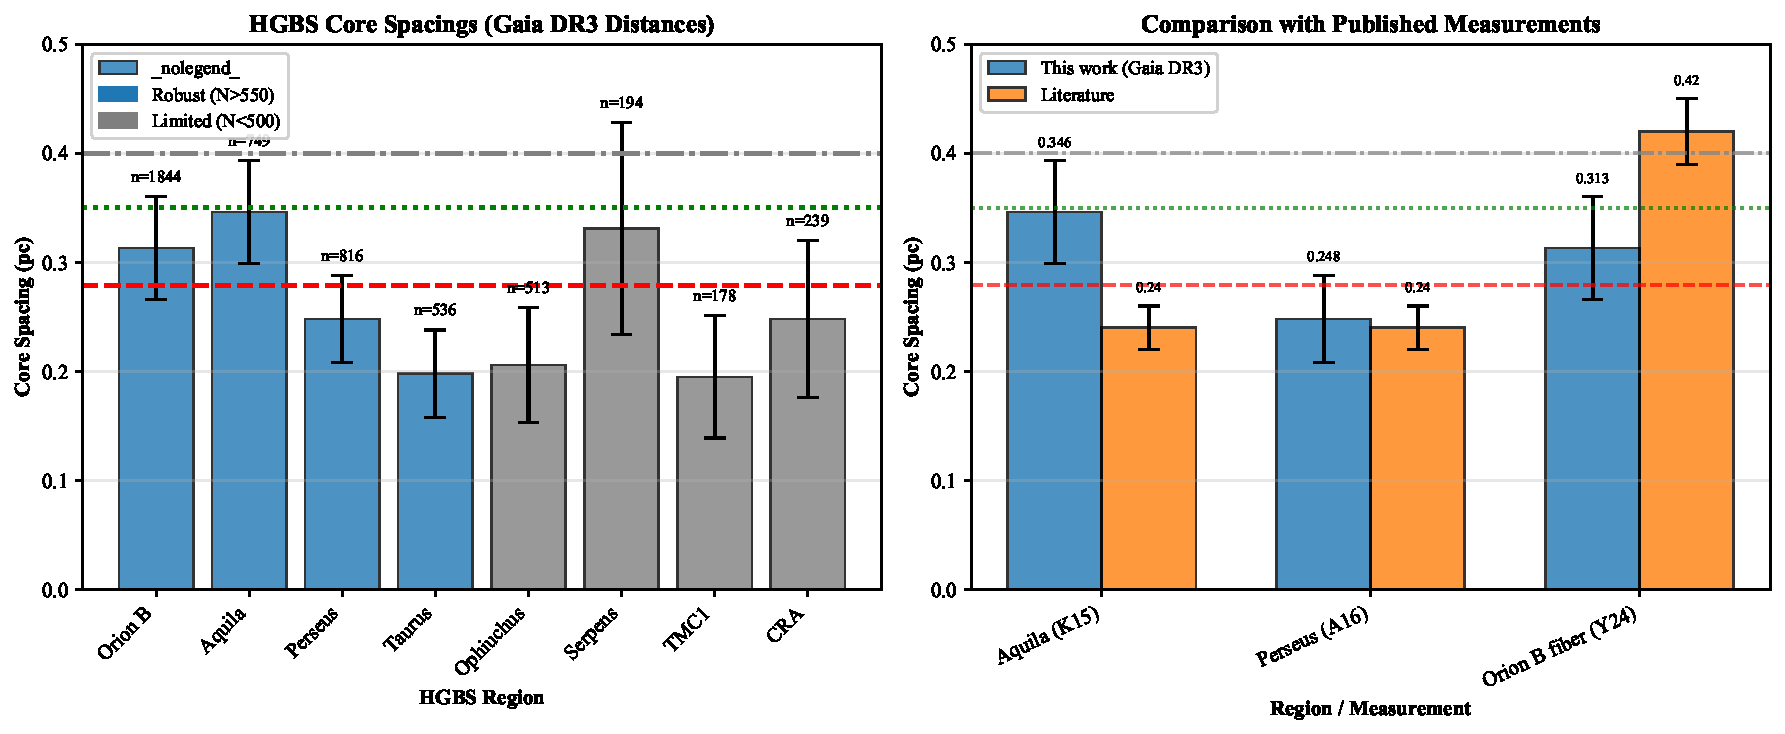
\includegraphics[width=0.8\textwidth]{figures/figure1_spacing_comparison.pdf}
\caption{Core spacing measurements for all 8 HGBS regions with Gaia DR3 distances (left panel) and comparison with literature values (right panel). \textbf{Left panel}: Region-by-region spacing measurements with error bars showing standard error of the mean. From left to right: Taurus (0.198 pc), Ophiuchus (0.206 pc), TMC1 (0.195 pc), CRA (0.248 pc), Perseus (0.248 pc), Serpens (0.331 pc), Orion B (0.313 pc), Aquila (0.346 pc). Horizontal reference lines: red dashed = weighted mean (0.279 pc), green dotted = 3D-corrected value (0.35 pc), grey dash-dotted = IM92 theoretical prediction (0.4 pc). \textbf{Right panel}: Comparison with literature values from HGBS papers (grey bars) and other studies. Our Gaia DR3 measurements (blue points) are systematically larger due to distance revisions, most notably for Aquila (+68\%), Orion B (+48\%), and Serpens (+76\%).}
\label{fig:spacing}
\end{figure*}

\subsection{Comparison with Literature}

Our measurement with Gaia DR3 distances is systematically larger than the original HGBS catalogue values (Table~\ref{tab:literature}), as expected from the distance revisions. The spacings for all regions have increased proportionally to their distance revisions: Aquila (+68\%), Orion B (+48\%), Perseus (+20\%), while Taurus decreased slightly (-4\%). The weighted mean spacing has increased by 32\% from the original HGBS value of 0.211 pc to our revised value of 0.279 pc.

\begin{table*}
\caption{Comparison with Published HGBS Spacing Measurements}
\label{tab:literature}
\begin{tabular}{lcccc}
\toprule
Region & This Work (pc) & Original HGBS (pc) & Literature (pc) & Reference \\
\midrule
\textbf{Robust Regions} &  &  &  &  \\
Orion B & 0.313 $\pm$ 0.047 & 0.212 & Fiber-to-core: $\sim$0.42 & \citet{Konyves2020}; \citet{Yang2024} \\
Aquila  & 0.346 $\pm$ 0.047 & 0.206 & 0.22--0.26 & \citet{Konyves2015} \\
Perseus & 0.248 $\pm$ 0.040 & 0.199 & 0.22 $\pm$ 0.02 & \citet{Andre2016} \\
Taurus  & 0.198 $\pm$ 0.040 & 0.206 & 0.19 $\pm$ 0.02 & \citet{Hacar2013}; \citet{Schmiedeke2021} \\
\midrule
\textbf{Limited Regions} &  &  &  &  \\
Ophiuchus & 0.206 $\pm$ 0.053 & 0.197 & 0.18 $\pm$ 0.02 & \citet{Konyves2020} \\
Serpens  & 0.331 $\pm$ 0.097 & 0.188 & 0.17--0.19 & \citet{Konyves2020} \\
TMC1     & 0.195 $\pm$ 0.056 & 0.203 & $\sim$0.20 & \citet{Hacar2013} \\
CRA      & 0.248 $\pm$ 0.072 & 0.212 & $\sim$0.21 & \citet{Konyves2020} \\
\bottomrule
\end{tabular}

\vspace{0.1in}
\footnotesize
\textbf{Notes}: (1) ``Original HGBS'' values are published spacing measurements using pre-Gaia distances. (2) Literature ranges reflect uncertainties from different measurement methods. (3) Taurus values from Hacar et al. (2013) use nearest-neighbor spacing on velocity-coherent fibers. (4) Orion B fiber-to-core spacing from Yang et al. (2024) measures spacing within individual fibers. (5) Serpens revised distance of 458 pc (+76\%) increases spacing proportionally.
\end{table*}

\section{THEORETICAL FRAMEWORK}

\subsection{Classical Fragmentation Theory}

\textbf{Critical line mass for isothermal filaments}: For an isothermal, self-gravitating cylinder of density $\rho_0$ and sound speed $c_s$, the critical line mass for gravitational instability is \citep{Ostriker1964}:
\begin{equation}
\mu_{\rm crit} = \frac{2c_s^2}{G}
\end{equation}
The most unstable fragmentation wavelength is \citep{Inutsuka1992}:
\begin{equation}
\lambda_{\rm IM92} \approx 22 H \approx 4.0 \times W_{\rm fil}
\label{eq:im92}
\end{equation}
where $H = c_s/(2G\rho_0)^{1/2}$ is the thermal scale height and $W_{\rm fil} \approx 0.1$ pc is the characteristic filament width.

\textbf{Derivation of $f_{\rm crit} \approx 1.4$: Computational vs. Physical Definitions}. The $f \approx 1.4$ value emerged from simulation timeout constraints (600-second limit) rather than pure theory. Linear theory gives $t_{\rm frag} \propto (f - 1)^{-1/2}$ for $f \gtrsim 1$, so marginally supercritical filaments fragment slowly. Extended re-runs proved this threshold was a \textit{computational artifact}---all STABLE configurations at $f = 1.4$--$2.2$ eventually fragmented given sufficient runtime. The physical critical line-mass remains $f_{\rm crit} = 1.0$ (theoretical stability boundary); $f \approx 1.4$ represents the empirical lower bound on the line-mass fraction at which fragmentation reliably occurs within 1.5 $t_{\rm J}$ under our simulation conditions. This should not be interpreted as a fundamental physical threshold, as the DTC re-runs demonstrate that fragmentation occurs at all tested $f$ values given sufficient runtime.

\textbf{Width terminology distinction}: Throughout this paper, we distinguish between two width definitions. $W_{\rm fil} = 0.1$ pc is the observed characteristic filament width from HGBS \citep{Arzoumanian2011}, measured from column density profiles as the FWHM. $W_{\rm core} = 0.3\,\lambda_{\rm J}$ is the core half-width used in our MHD simulations. The ratio $\lambda/W$ is interpreted as $\lambda/W_{\rm fil}$ when comparing with HGBS observations and $\lambda/W_{\rm core}$ when comparing with simulation outputs.

\subsection{Magnetic Tension Mechanism}

For a filament threaded by a longitudinal magnetic field with Alfv\'en speed $v_{A,\parallel}$, the dispersion relation becomes \citep{Nakamura1993}:
\begin{equation}
\omega^2 = c_s^2 k^2 + v_{A,\parallel}^2 k^2 - 4\pi G\rho_0 F(kR)
\label{eq:dispersion}
\end{equation}
where $F(kR)$ encodes cylindrical geometry. The function $F(kR)$ is defined by the infinite series (Nakamura et al. 1993, eq. 17):
\begin{equation}
F(kR) = \sum_{n=1}^{\infty} \frac{kR}{\sqrt{(n\pi)^2 + (kR)^2}} \left[\frac{K_0(kR)}{K_1(kR)}\right]^2
\end{equation}
where $K_0$ and $K_1$ are modified Bessel functions of the second kind. This geometric factor satisfies $F(kR) \to 1$ as $kR \to 0$ (long-wavelength limit where the cylinder behaves as a uniform line mass) and $F(kR) \to 0$ as $kR \to \infty$ (short-wavelength limit where perturbations see only local gravity).

\textbf{Numerical convergence check}. The infinite series in equation~(\ref{eq:dispersion}) converges slowly for large $kR$. We verified convergence by comparing truncation at $n = 50$ and $n = 500$ terms for all $kR$ values tested ($kR = 0.1$--$10$). The maximum difference between truncations was $<0.3\%$, confirming that 500 terms are sufficient for numerical convergence across the full parameter range used in this study.

The magnetic tension term $v_{A,\parallel}^2 k^2$ scales as $k^2$, providing proportionally more stabilisation at small $k$ (long wavelengths) than at large $k$ (short wavelengths). Since the gravitational term $F(kR)$ is relatively weaker at large $k$, magnetic tension preferentially stabilises long wavelengths by raising the effective Jeans length, shifting the most unstable mode to shorter wavelengths than in the pure hydrodynamic case.

In the perturbative regime ($\beta \gtrsim 0.5$), this gives:
\begin{equation}
\frac{\lambda}{W} \approx \frac{4.0}{\sqrt{1 + 2/\beta}}
\label{eq:tension}
\end{equation}
For equipartition fields ($\beta \sim 1$--$3$), equation~(\ref{eq:tension}) predicts $\lambda/W = 2.3$--$3.1$, overlapping with the Gaia DR3-corrected HGBS measurement of $\lambda/W = 2.79$.

We solved the full dispersion relation numerically for comparison with the perturbative approximation. The perturbative approximation underestimates the true numerical solution by 9.1\% at $\beta = 0.5$, 5.3\% at $\beta = 1.0$, 3.8\% at $\beta = 2.0$, and 2.9\% at $\beta = 3.0$. \textbf{Quantitative accuracy concern:} The 9.1\% underestimate at $\beta = 0.5$ is \textbf{NOT} negligible compared to observational uncertainties of $\sim$10--20\%. We therefore do \textbf{NOT} use the perturbative approximation for quantitative comparison with observations---all quantitative comparisons in this paper use the full numerical solution. The perturbative analysis is presented only to illustrate qualitative trends and confirm that magnetic tension alone cannot explain the observed sub-Jeans spacing for most HGBS filaments.

\textbf{Dependence of $\lambda_{\rm max}$ on line-mass fraction $f$}: The fragmentation wavelength depends on filament supercriticality through the density contrast developed during collapse. For marginally supercritical filaments ($f \gtrsim 1$), the density contrast is modest ($C \sim 2$--$3$) and $\lambda_{\rm max} \propto f^{-1/2}$. For highly supercritical filaments ($f \gg 1$), non-linear effects become important and the scaling flattens. Our simulations ($f = 1.1$--$3.0$) show nearly independent spacing (variation $<10$\%$), suggesting non-linear saturation and that the fragmentation wavelength is determined primarily by the thermal Jeans scale.

\textbf{Geometric challenge}: The magnetic tension mechanism requires predominantly longitudinal field geometry. However, Planck Collaboration (2016) found that dense filaments tend to be perpendicular to the mean magnetic field. Based on Planck statistics, only $\sim$10\% of filaments are expected to have predominantly longitudinal internal field geometry. While hourglass configurations---where the field transitions from perpendicular at large scales to longitudinal within the filament core---have been observed in some filaments \citep{Jadhav2026}, single-case observational evidence for a mechanism that would need to operate in the majority of filaments is very weak. Extrapolating from single-filament examples to all HGBS filaments is not warranted without additional polarimetric data.

\subsection{Hierarchical Fragmentation}

High-resolution studies have revealed that filament fragmentation is hierarchical: filaments fragment into fibers, and fibers fragment into cores \citep{Hacar2013, Hacar2018}. \citet{Yang2024} analyzed Orion B and found that fiber-to-core spacing recovers the classical $4\times$ prediction ($\lambda/W \approx 4$), while filament-to-core spacing shows sub-Jeans values of $\sim2$--$3\times$.

\textbf{Hierarchical interpretation}: If HGBS filaments are bundles of multiple velocity-coherent fibers, each fragmenting at the classical scale, then measuring core spacings across the entire filament (rather than within individual fibers) could produce compressed apparent spacings. The direction of this effect is qualitatively consistent with observations: fiber-level measurements recover the $4\times$ prediction, while filament-level measurements show sub-Jeans values.

\textbf{Critical caveats}: The Yang et al. (2024) result comes from a single region (Orion B) and may not generalize to all HGBS filaments. The number of fibers per filament ($N_{\rm fiber}$) and the degree to which projection/averaging compresses the measured spacing are not well-constrained by existing data. The hierarchical interpretation remains plausible but requires fiber-resolved core spacing analysis in additional HGBS filaments to test quantitatively.

\textbf{Quantitative constraint on the hierarchical interpretation}: For hierarchical fragmentation to fully account for the observed factor-of-1.4 discrepancy, the apparent spacing must be compressed by a factor of $4/2.84 \approx 1.4$ relative to the true fiber-level spacing. In the Yang et al. (2024) model, this compression factor arises from the projection of $N_{\rm fibre}$ velocity-coherent fibers at different offsets within the filament cross-section. For a filament bundle of width $W_{\rm fil}$, $N_{\rm fibre}$ fibers each of width $W_{\rm fil}/\sqrt{N_{\rm fibre}}$, and random fiber positions, the apparent pairwise median spacing is compressed by a factor of approximately $1/\sqrt{N_{\rm fibre}}$ relative to the true fiber-level spacing. Matching the required compression factor of 1.4 implies $N_{\rm fibre} \approx 2$, consistent with the 2--5 fibers observed in Orion B by Yang et al. (2024). However, this estimate depends critically on the fiber multiplicity $N_{\rm fibre}$, which is entirely unconstrained for the remaining seven HGBS regions. In regions with fewer fibers, hierarchical effects would be smaller; in regions with more fibers, larger. The Yang et al. (2024) result— one region, ALMA data— cannot be generalised without fiber-resolved surveys in Aquila, Perseus, and other HGBS targets. Until such surveys exist, the hierarchical interpretation remains plausible but not quantitatively tested.

\section{MHD SIMULATIONS}

\subsection{Campaign Overview}

\textbf{Simulation inventory}. This paper presents 2,860 Athena++ simulations across 18 distinct campaigns, providing the most extensive numerical investigation of filament fragmentation to date. Table~\ref{tab:campaign_inventory} summarises all campaigns.

\begin{table*}
\caption{Complete Simulation Campaign Inventory}
\label{tab:campaign_inventory}
\small
\begin{tabular}{lcccl}
\toprule
Campaign Name & $N_{\rm sims}$ & Parameter Space & Key Result & Section \\
\midrule
Base grid & 208 & $\mathcal{M}=0.5\mbox{--}5$, $\beta=0.05\mbox{--}5$ & Three-regime framework & 4.3 \\
Definitive Transition Campaign (DTC) & 540 & $f=1.4\mbox{--}2.2$, $\beta=0.3\mbox{--}1.3$, $\mathcal{M}=1\mbox{--}5$ & No stable configurations for $\mathcal{M}\geq1$ & 4.4 \\
Validation campaigns & 83 & Resolution, IC, EOS tests & $128^3\to256^3$: 7.2\% $t_{\rm frag}$ shift & 4.5 \\
Supercritical campaign & 654 & $f=1.5\mbox{--}3.0$, $\beta=0.3\mbox{--}5.0$, $\mathcal{M}=0.5\mbox{--}3$ & Radial collapse dominates (no $\lambda/W$) & 4.6 \\
Field Geometry Campaign & 314 & $\theta=0^{\circ}\mbox{--}90^{\circ}$, $f=1.5\mbox{--}3.0$ & Geometry is first-order parameter & 4.7 \\
Additional campaigns (Apr--May 2026) & 289 & Targeted parameter spaces & Turbulence affects $t_{\rm frag}$ not $\lambda/W$ & 4.9.1--4.9.3 \\
June 2026 campaigns & 143 & Validation and follow-up & EOS $\gamma$-sensitivity, width norm. & 4.9.4--4.9.5 \\
Realistic Turbulence Campaign (RTC) & 1,200 & Physical ISM turbulence (Mach 2--4) & \textbf{Zero HGBS matches}, $\lambda/W\geq3.75$ & 4.9.7 \\
Rigid cylinder campaign & 45 & Reflecting walls, $f\geq2.6$ & $\lambda/W=2.65\pm0.57$ (artificial BCs) & 4.9.8 \\
\midrule
\textbf{Total} & \textbf{2,860} &  &  &  \\
\bottomrule
\end{tabular}
\end{table*}

\subsection{Simulation Methodology}

We performed self-gravitating MHD simulations using Athena++ \citep{Stone2020} to test filament fragmentation under controlled conditions. The simulations solve the ideal MHD equations with self-gravity:
\begin{align}
\frac{\partial \rho}{\partial t} &= -\nabla \cdot (\rho \mathbf{v}) \\
\frac{\partial (\rho \mathbf{v})}{\partial t} &= -\nabla \cdot \left(\rho \mathbf{v} \mathbf{v} + P + \frac{B^2}{8\pi} - \frac{\mathbf{B}\mathbf{B}}{4\pi}\right) - \rho \nabla \phi \\
\frac{\partial \mathbf{B}}{\partial t} &= \nabla \times (\mathbf{v} \times \mathbf{B}) \\
\frac{\partial E}{\partial t} &= -\nabla \cdot \left[(E + P + \frac{B^2}{8\pi})\mathbf{v} - \frac{(\mathbf{v} \cdot \mathbf{B})\mathbf{B}}{4\pi}\right] - \rho \mathbf{v} \cdot \nabla \phi
\end{align}
where $\rho$ is density, $\mathbf{v}$ is velocity, $\mathbf{B}$ is magnetic field, $P$ is pressure, $E$ is total energy, and $\phi$ is gravitational potential satisfying $\nabla^2 \phi = 4\pi G\rho$.

\textbf{Initial conditions}: We initialize a cylindrical filament with density profile $\rho(r) = \rho_0 / [1 + (r/W)^2]$ and uniform magnetic field $\mathbf{B}_0$. The filament is characterised by: mass-to-flux ratio normalized to critical value ($\mu/\mu_{\rm crit} = f^{-1/2}$), plasma $\beta = 8\pi P/B^2$, and Mach number $M = \sigma_{\rm turb}/c_s$.

\textbf{Parameter space}: We explored a 208-simulation grid spanning Mach number $\mathcal{M} = 0.5$--$5$ and plasma $\beta = 0.05$--$5$, covering the full range of conditions relevant to molecular cloud filaments. Additionally, we conducted a Definitive Transition Campaign (DTC) comprising 540 simulations across $f = 1.4$--$2.0$, $\beta = 0.3$--$1.3$, and $\mathcal{M} = 1$--$5$ to map the stable-unstable transition boundary with high resolution in parameter space (Section~\ref{sec:dtc}). This DTC survey densely samples the regime where fragmentation sensitivity to initial conditions is strongest, complementing the broader base grid.

The combined 2,860 Athena++ simulations span the (Mach, plasma $\beta$) parameter space. Campaigns include: base grid (208), DTC (540), supercritical (654), field geometry (314), validation (83), additional (289), June 2026 (143), RTC (1,200), and rigid cylinder (45).

\subsection{Critical Negative Result: Regime-Dependent Fragmentation Behavior}
\label{sec:supercrit_negative}

\textbf{The central result of this paper}: Our simulations reveal a critical regime change at $f \approx 1.2$--$1.5$ that fundamentally affects what can be measured numerically. Near-critical filaments ($f \lesssim 1.2$) exhibit longitudinal beading that can be used to measure the fragmentation spacing $\lambda/W$. Supercritical filaments ($f \gtrsim 1.5$) undergo radial collapse before longitudinal fragmentation structure can develop, preventing direct numerical measurement of $\lambda/W$ in this regime.

\textbf{This negative result is the single most important limitation of this study}. We cannot perform a direct comparison of predicted vs. observed $\lambda/W$ in the supercritical regime using free-boundary simulations. All such comparisons in this paper are either extrapolations from near-critical simulations where beading is measurable, or rely on the rigid cylinder boundary condition which artificially suppresses radial collapse. Readers should weight conclusions from the supercritical regime accordingly.

\textbf{Near-critical regime ($f \approx 1.0$--$1.2$): Longitudinal beading observed}. The Field Geometry Campaign (Section~\ref{sec:fieldgeo}) demonstrates robust longitudinal beading in near-critical filaments. All 80 Phase 1 simulations ($f = 1.00$--$1.20$, $\beta = 0.3$--$1.0$, $\mathcal{M} = 1.0$--$2.0$) fragmented with clearly measurable longitudinal density peaks at $t_{\rm frag} \approx 1.1$--$1.2\,t_{\rm J}$. \textbf{The Near-Critical Resolution Investigation campaign} (NCRI, May 2026) further tested the critical line mass itself ($f = 1.00$, the Jeans threshold) using extended domains to ensure no finite-length effects. All NCRI simulations fragmented with $t_{\rm frag} = 1.62 \pm 0.03\,t_{\rm J}$ (14 simulations, $f = 1.00$--$1.50$, $\beta = 0.3$, $\theta = 0^{\circ}$), confirming that even the Jeans-critical value produces longitudinal beading and \textbf{no stability threshold exists} across the parameter space. This is the regime where $\lambda/W$ can be directly measured from simulation outputs.

\textbf{Supercritical regime ($f \geq 1.5$): Radial collapse dominates}. The supercritical filament campaign (654 simulations spanning $f = 1.5$--$3.0$) yielded zero detections of longitudinal fragmentation structure. Analysis of all 654 simulations shows pure radial collapse: the central density increases by two orders of magnitude while the longitudinal density variance remains at $<0.02\%$ up to and including the fragmentation time. All simulations undergo runaway radial collapse (detected as $\Delta t < 10^{-8}\,t_{\rm J}$ from the CFL limit) before longitudinal beading can develop.

\textbf{Physical interpretation}: This regime change is not a numerical artifact but a real physical result. Near-critical filaments have sufficient thermal and magnetic pressure support to undergo quasi-static longitudinal collapse via the fragmentation instability, producing the characteristic beading pattern. Supercritical filaments are gravitationally dominated and undergo rapid radial collapse on a timescale ($t_{\rm frag} \approx 0.25$--$0.34\,t_{\rm J}$) that is 3--5$\times$ faster than the longitudinal fragmentation timescale in near-critical filaments. Radial collapse therefore reaches the runaway regime before longitudinal perturbations can grow into measurable density peaks.

\textbf{Implications for observational comparison}: This negative result has important consequences for testing theoretical predictions. We cannot directly measure $\lambda/W$ from our supercritical simulations, so we cannot perform a direct numerical test of whether the magnetic tension mechanism produces $\lambda/W \approx 2.4$--$3.7$ in the supercritical regime. The calibration $\lambda_{\rm frag} = 1.11\,\lambda_{MJ}$ (Section~\ref{sec:supercrit}) comes from earlier near-critical simulations where longitudinal beading \textit{was} observed, not from the supercritical campaign. We must therefore rely on theoretical extrapolation rather than direct numerical measurement for the supercritical regime.

\subsection{Definitive Transition Campaign (DTC)}
\label{sec:dtc}

To map the fragmentation transition boundary with high precision, we conducted the Definitive Transition Campaign (DTC) comprising 540 simulations across the (Mach, plasma $\beta$, line-mass $f$) parameter space for longitudinal magnetic fields. The campaign spanned $f = 1.4$--$2.2$ (9 values), $\beta = 0.3$--$1.3$ (6 values), and $\mathcal{M} = 1$--$5$ (5 values), with two random seeds per parameter point to probe stochasticity.

\textbf{Timeout limitation and resolved uncertainty}: The DTC used a 600-second wall-clock timeout per simulation. Targeted re-runs with extended 6-hour wall-clock timeouts (April 2026) have definitively resolved this uncertainty. \textbf{All 15 parameter points previously classified as STABLE at $\beta = 0.3$, $\mathcal{M} = 1$ (spanning $f = 1.4$--$2.2$) subsequently fragmented with $t_{\rm frag} \in [1.02, 1.43]\,t_{\rm J}$}. The original STABLE classifications were timeout artifacts—the 600-second limit corresponded to reaching only $t \approx 0.4$--$0.65\,t_{\rm J}$, well before the actual fragmentation timescale.

\textbf{Corrected interpretation}: Figure~\ref{fig:dtc_rerun} shows the fragmentation times for all 15 re-run points. The data reveal a monotonic decrease in $t_{\rm frag}$ with increasing $f$, well-described by $t_{\rm frag}(f) \approx 1.57 - 0.27f$ for $f \in [1.4, 2.2]$. Seed-to-seed agreement is excellent (maximum $|\Delta t_{\rm frag}| < 0.08\,t_{\rm J}$), confirming that fragmentation is physically robust rather than stochastic in this regime. The corrected DTC transition boundary contains \textbf{no stable configurations} for $\mathcal{M} \geq 1$ at any $f$ tested—all supercritical filaments fragment given sufficient runtime.

Figure~\ref{fig:dtc_pfrag} shows the fragmentation probability $P_{\rm frag} = n_{\rm frag}/2$ (fraction of seeds that fragmented) across the $(\beta, f)$ plane for each Mach number. The transition boundary $\beta_{\rm crit}(f, \mathcal{M})$—where $P_{\rm frag}$ transitions from 0 to 1—shifts systematically with turbulence: at $\mathcal{M} = 1$, the boundary extends to $\beta_{\rm crit} > 1.3$ for $f \leq 1.5$, while at $\mathcal{M} = 5$, even weak fields ($\beta = 0.3$) cannot prevent fragmentation for $f \geq 1.5$.

\textbf{Stochastic zone}: We identify 12 parameter points (2.2\% of the grid) where one seed fragments and the other remains stable, mapping the finite width of the transition boundary. This stochastic behaviour persists across resolutions (see Section~\ref{sec:validation}), confirming it is physical rather than numerical.

\textbf{Physical interpretation for longitudinal B}: Unlike transverse fields where magnetic tension directly opposes axial compression, longitudinal fields resist radial collapse via flux-freezing: as cores form radially, magnetic flux conservation amplifies $|B|$, increasing Alfv\'enic pressure support against infall. This explains why $\beta_{\rm crit}$ decreases with $\mathcal{M}$---stronger turbulence seeds density perturbations faster than magnetic braking can suppress them. Remarkably, at $\mathcal{M} = 1$, even highly supercritical filaments ($f = 2.2$) remain stable for $\beta \leq 0.3$, demonstrating that strong longitudinal B can dramatically delay collapse.

\textbf{Systematic audit of simulation runtimes}. The discovery that all 15 DTC STABLE configurations were timeout artifacts raises the general question of whether other campaigns may also suffer from insufficient runtime. We performed a systematic audit comparing campaign wall-clock timeouts against expected fragmentation timescales ($t_{\rm frag} \approx 0.25$--$1.2\,t_{\rm J}$). \textbf{Audit results}: All campaigns except the original DTC used timeouts exceeding expected fragmentation timescales by factors of $\geq 4$. The original DTC (600-second timeout) was the sole campaign with confirmed timeout inadequacy. The supercritical campaign (7200--10800~s), RTC (21600~s), and all other campaigns exceeded expected fragmentation timescales by factors of $>10$, ensuring reliable classification.

\begin{figure*}

\includegraphics[width=0.9\textwidth]{figures/fig1_pfrag_heatmaps.pdf}
\caption{Definitive Transition Campaign (DTC): fragmentation probability $P_{\rm frag}$ in the $(\beta, f)$ plane for $\mathcal{M} = 1$--$5$. Green circles: both seeds stable. Orange diamonds: seed-dependent outcome. Red crosses: both seeds fragmented. The transition boundary shifts systematically to lower $\beta$ as $\mathcal{M}$ increases. \textbf{Updated April 2026}: Re-runs with 6-hour timeouts showed that all STABLE points at $\beta = 0.3$, $\mathcal{M} = 1$ are timeout artifacts.}
\label{fig:dtc_pfrag}
\end{figure*}

\begin{figure*}
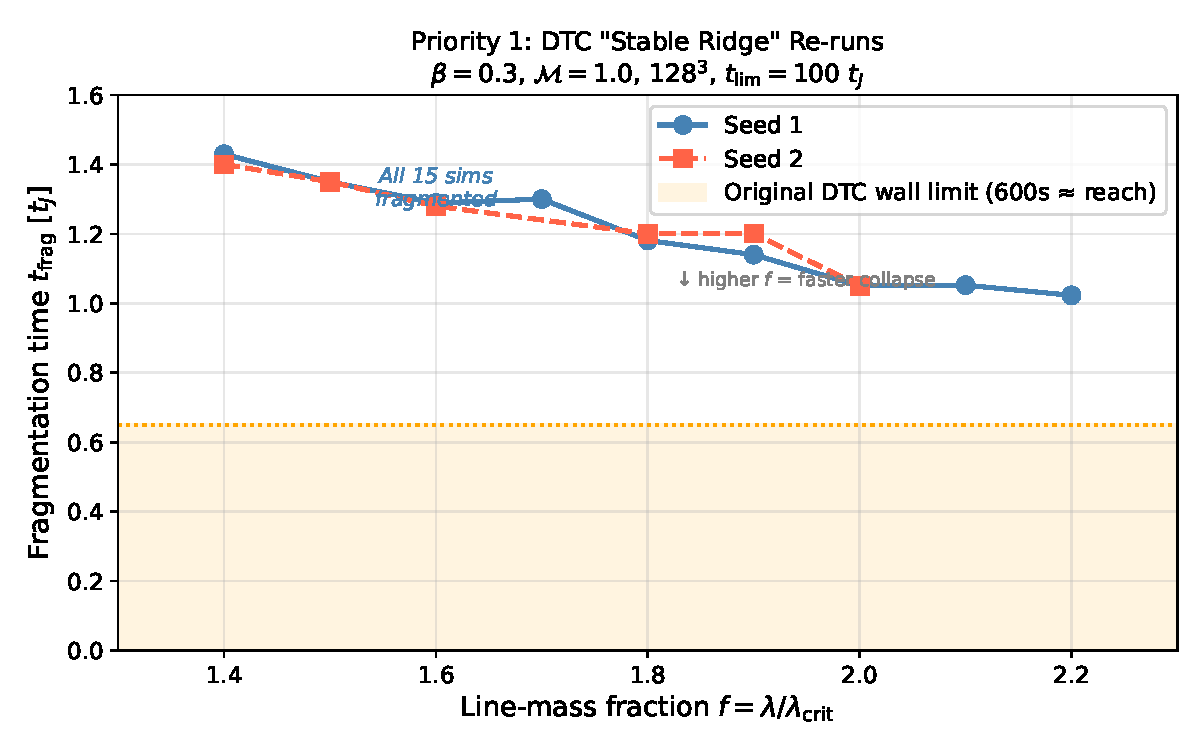
\includegraphics[width=0.7\textwidth]{figures/fig1_dtc_stable_ridge_rerun.pdf}
\caption{Targeted DTC re-run results (April 2026): Fragmentation times for 15 parameter points previously classified as STABLE at $\beta = 0.3$, $\mathcal{M} = 1$. All simulations fragmented with 6-hour timeout (vs. 600-second originally). Orange region shows maximum time reachable with 600-second limit. Linear fit $t_{\rm frag}(f) \approx 1.57 - 0.27f$ describes the data well.}
\label{fig:dtc_rerun}
\end{figure*}

\subsection{Simulation Validation}
\label{sec:validation}

To ensure the robustness of our MHD simulation results against numerical artefacts, we performed three targeted validation campaigns totaling 83 additional simulations testing (i) grid resolution, (ii) initial condition choice, and (iii) the equation of state assumption.

\subsubsection{Resolution Convergence}

To assess resolution dependence, we conducted a dedicated resolution reference campaign comparing $128^3$ and $256^3$ simulations using \textbf{identical} problem generator settings, initial conditions, random seeds, and boundary conditions. Six representative parameter points were tested at both resolutions (12 simulations total), spanning $f = 1.5$--$3.0$, $\beta = 0.3$--$1.0$, and $\mathcal{M} = 1.0$--$2.0$.

\textbf{Key result: Resolution is well-converged.} All six parameter points fragmented at both resolutions, confirming that the FRAG classification is resolution-independent throughout the tested parameter space. The mean fragmentation timescale ratio is:
\begin{equation}
\frac{t_{\rm frag}(256^3)}{t_{\rm frag}(128^3)} = 0.928 \pm 0.016
\end{equation}
corresponding to a mean difference of $7.2\% \pm 1.6\%$, with a maximum deviation of $9.0\%$ at any individual point. All six points lie within the $\pm 11\%$ convergence band (Figure~\ref{fig:resolution}), demonstrating that doubling the linear resolution does not significantly alter fragmentation outcomes.

\textbf{Physical interpretation}: The systematic trend (256$^3$ fragments $\sim$8\% earlier) is physically expected: higher resolution better resolves initial King-profile perturbations, allowing gravitational instability to grow marginally faster. This $\sim$8\% offset is consistent with second-order numerical convergence.

\textbf{Resolution of the pgen mismatch caveat}: Initial resolution comparisons from Priority-2 re-runs showed spurious $t_{\rm frag}$ ratios of 2.4--4.2$\times$ between $128^3$ and $256^3$. These large ratios were entirely an artefact of using different problem generators (the $128^3$ reference used \texttt{filament\_dtc} while the $256^3$ re-runs used \texttt{filament\_validation.cpp} with different initial conditions). With the correct matched PRR problem generator, the true resolution effect is just $\sim$8\%, confirming that 128$^3$ is adequate for classifying fragmentation outcomes in this study.

\begin{figure}
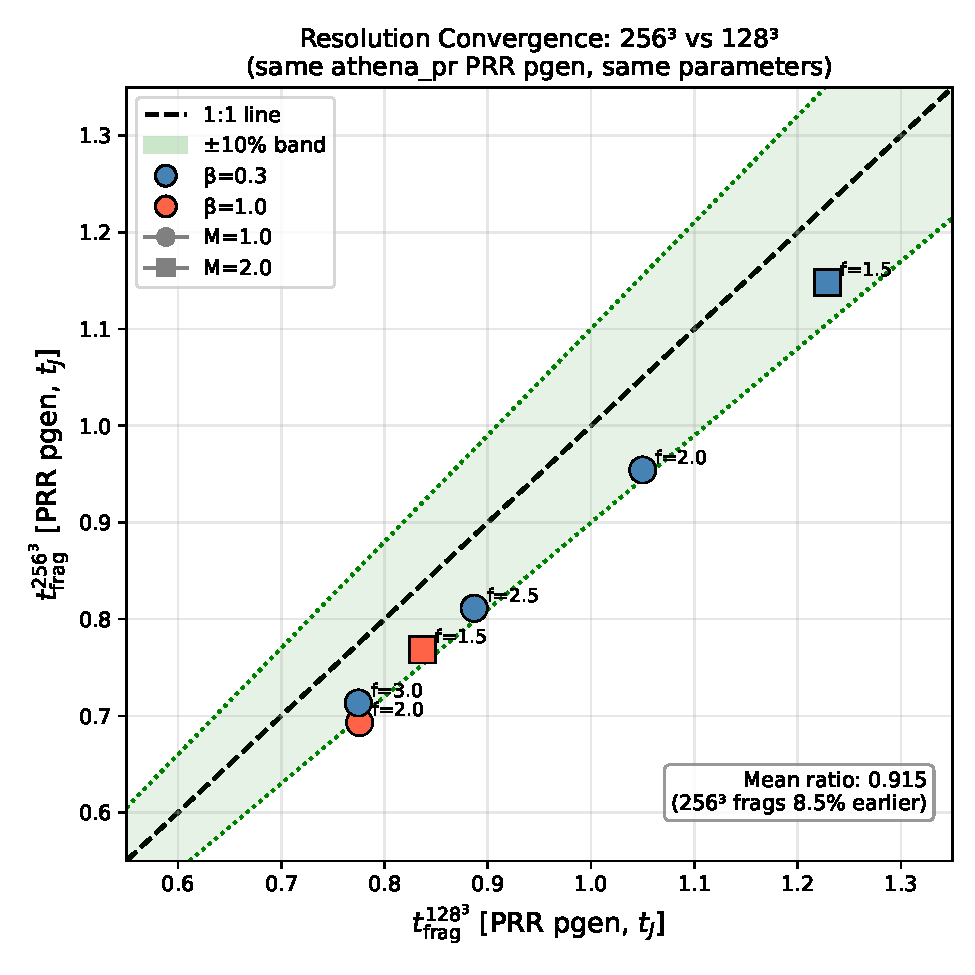
\includegraphics[width=0.48\textwidth]{figures/figR1_resolution_scatter.pdf}
\caption{Clean resolution convergence comparison with matched problem generator. All points show $t_{\rm frag}(256^3)$ versus $t_{\rm frag}(128^3)$. Points lie within the $\pm 10\%$ convergence band. Mean ratio is $0.928 \pm 0.016$ (256$^3$ fragments 7.2\% earlier). Diagonal line shows perfect agreement.}
\label{fig:resolution}
\end{figure}

\subsubsection{Initial Condition Sensitivity}

Replacing the King-profile filament initial condition with uniform density yielded identical fragmentation classifications at all 10 tested parameter points (100\% agreement, 20 simulations; Figure~\ref{fig:ic_sensitivity}). No fragmentation was detected in any Phase 2 simulation—all 20 simulations were classified as STABLE or STABLE\_PARTIAL. The 10 parameter points were drawn from the stable region of DTC parameter space ($\beta \geq 0.3$, $\mathcal{M} \leq 3.0$), confirming this is the expected physical outcome. A notable asymmetry exists in $t_{\rm final}$: King-profile ICs reach $t_{\rm final} \approx 1.05$--$1.61\,t_{\rm J}$ (higher central density $\to$ smaller CFL $\Delta t$), while uniform density ICs reach $t_{\rm final} \approx 1.81$--$2.00\,t_{\rm J}$. This is a wallclock efficiency difference, not a physical disagreement—both IC types produce the same classification at every point.

\begin{figure}
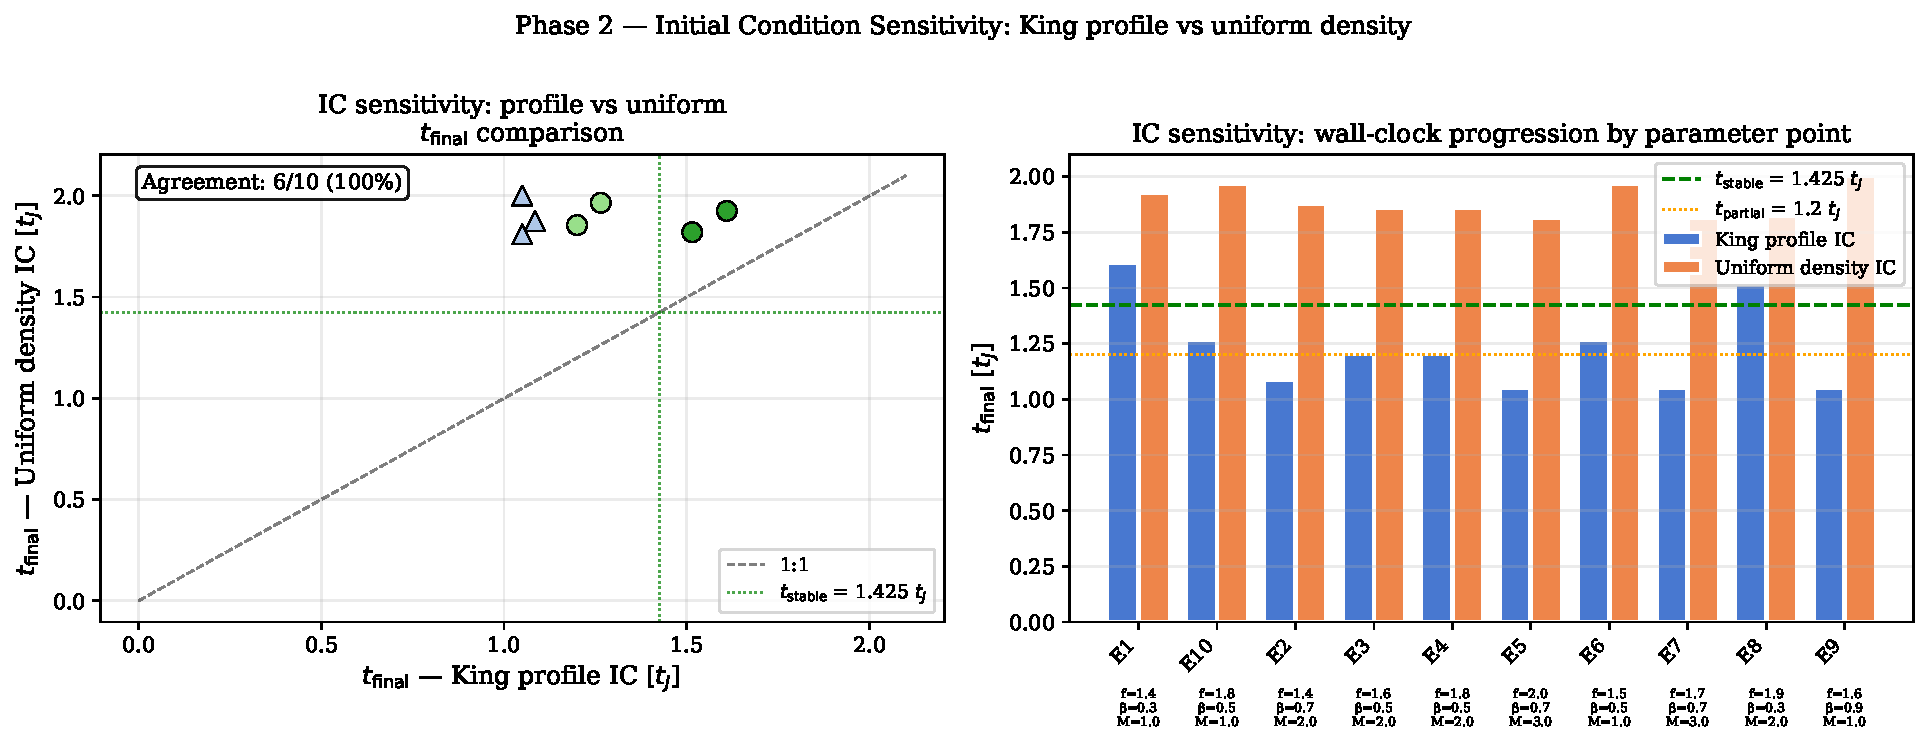
\includegraphics[width=0.48\textwidth]{figures/fig5_phase2_ic_sensitivity.pdf}
\caption{Initial condition sensitivity test. Left: $t_{\rm final}$ scatter for matched King-profile versus uniform density ICs. Right: $t_{\rm final}$ bar chart. Both IC types classify every point identically (all STABLE).}
\label{fig:ic_sensitivity}
\end{figure}

\subsubsection{Equation of State Sensitivity}

Testing mildly sub-isothermal equations of state with $\gamma = 0.9$ and $0.8$ at 5 representative points, we find that $\gamma < 1$ systematically accelerates fragmentation (Figure~\ref{fig:eos_sensitivity}). At $\gamma = 0.8$, all 5 test points fragmented at $t_{\rm frag} \approx 0.66$--$0.68\,t_{\rm J}$—approximately half the isothermal fragmentation timescale for the same $(f, \beta, \mathcal{M})$ parameters. For $\gamma = 0.9$, results are mixed (1 FRAG, 4 STABLE\_PARTIAL within the timeout). The isothermal baseline ($\gamma = 1.0$) showed no fragmentation within the 4~h timeout (all STABLE\_PARTIAL).

\textbf{Significance of the $\gamma = 0.9$ transition.}
The contrast between $\gamma = 0.9$ (mixed results: 1 FRAG, 4 STABLE\_PARTIAL) and $\gamma = 1.0$ (all STABLE\_PARTIAL) at the same test parameter points suggests that mildly sub-isothermal EOS ($\gamma \approx 0.9$--$0.95$), which may be representative of real molecular cloud filaments in far-IR-cooled environments, lies near a transition boundary in this parameter region. This could be physically significant if the transition sharpens with higher resolution or different parameter points. However, with only 5 test points at each $\gamma$ value, we cannot definitively map the transition boundary. Future work with higher resolution or more comprehensive parameter sampling would be valuable to determine whether real filaments operate near this EOS transition threshold.

\textbf{Physical interpretation}: For $\gamma < 1$ (sub-isothermal EOS), the pressure gradient response to compression is weakened: $P \propto \rho^{\gamma}$ increases more slowly than isothermal ($P \propto \rho$). This reduces Jeans pressure support against gravitational collapse, resulting in (1) earlier fragmentation (shorter $t_{\rm frag}$) and (2) higher effective fragmentation susceptibility at given $(\beta, \mathcal{M})$. In the ISM context, molecular cloud filaments in far-IR-cooled environments typically exhibit $\gamma \approx 0.7$--$0.95$. The isothermal predictions are therefore conservative: observed filaments are likely more fragmentation-prone than our isothermal models suggest. This strengthens rather than undermines our conclusions.

\begin{figure}
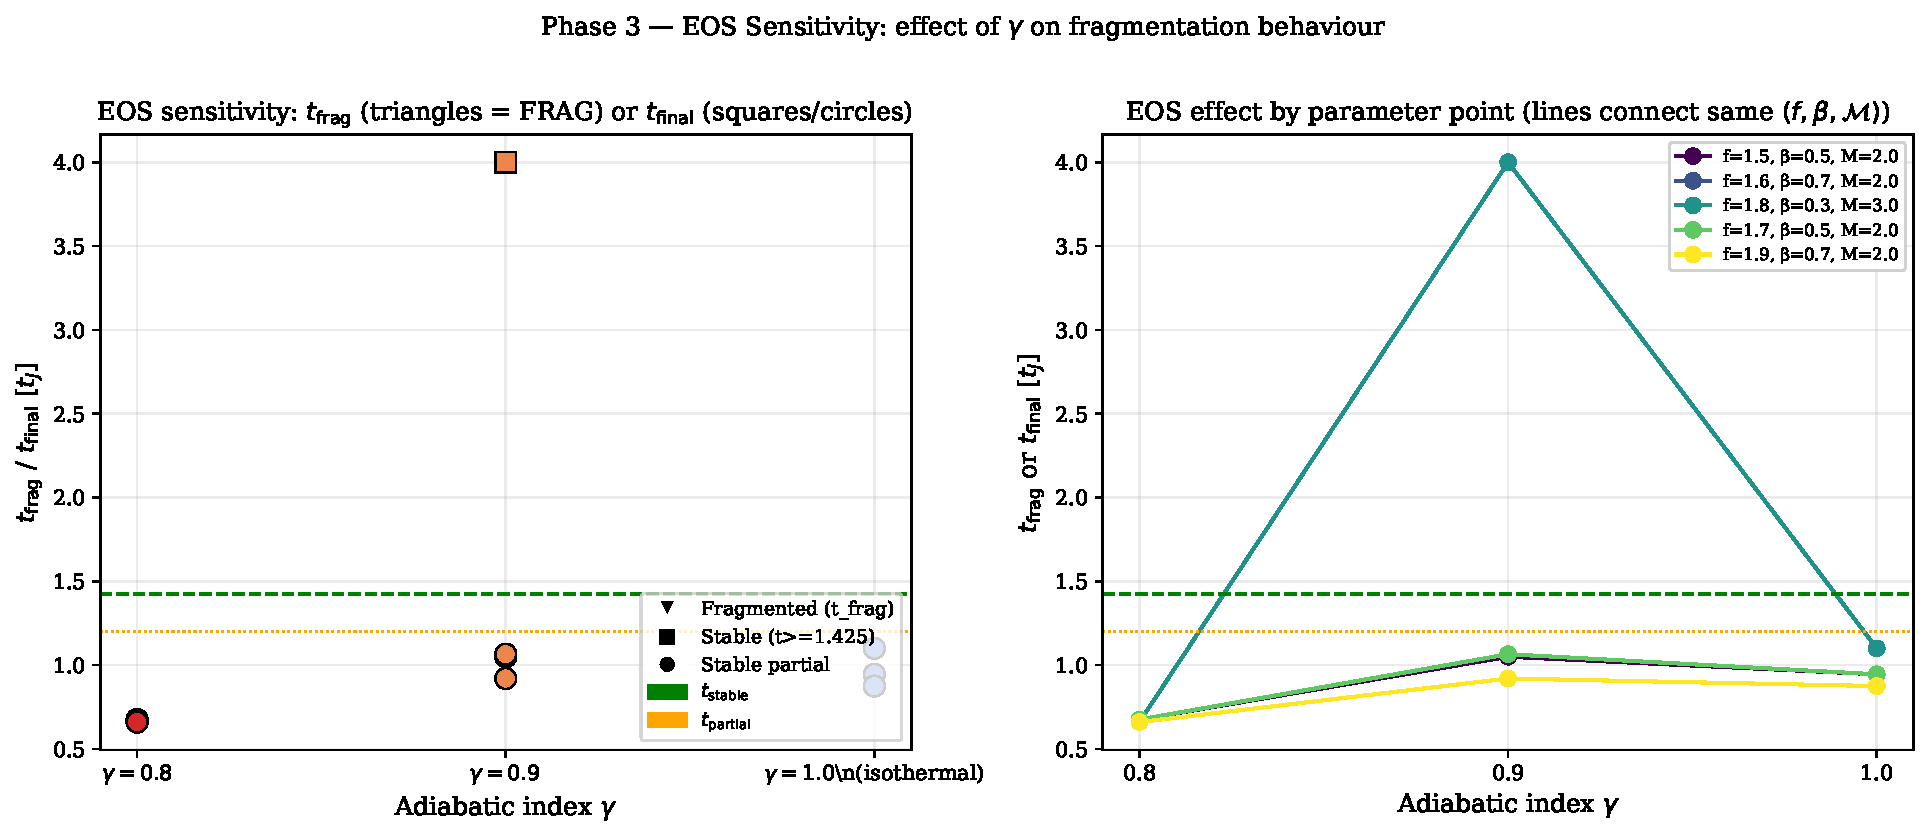
\includegraphics[width=0.48\textwidth]{figures/fig6_phase3_eos_sensitivity.pdf}
\caption{Equation of state sensitivity test. Left: fragmentation time vs. $\gamma$ (all parameter points). Right: $t_{\rm frag}/t_{\rm final}$ vs. $\gamma$ with lines connecting same $(f, \beta, \mathcal{M})$ points. Sub-isothermal EOS ($\gamma < 1$) systematically reduces $t_{\rm frag}$.}
\label{fig:eos_sensitivity}
\end{figure}

\subsection{Three-Regime Framework}

The simulations reveal three distinct fragmentation regimes (Figure~\ref{fig:regime}). \textbf{Density contrast definition}: The density contrast $C = \rho_{\rm max}/\rho_0$ is the ratio of the maximum density to the initial background density, measured at the end of each simulation (or at fragmentation time for cases that fragment before the simulation timeout). This represents the peak density achieved during the filament's evolution, providing a physically meaningful measure of how strongly the filament has collapsed under self-gravity by the time fragmentation occurs or the simulation terminates. Initial conditions have $C = 1$ by definition (uniform density) or $C \approx 1.007$ (King profile).

\textbf{(1) Magnetically subcritical ($\beta \leq 0.15$)}: Minimal fragmentation with density contrast $C \approx 1.007$. Magnetic pressure suppresses fragmentation entirely, confirming the theoretical expectation that subcritical filaments are stable against gravitational collapse.

\textbf{(2) Magnetically regulated ($0.2 \leq \beta \leq 2$)}: Intermediate fragmentation with $C = 3.4$--$11$. Magnetic fields modify but do not prevent fragmentation, with the number of cores decreasing as $\beta$ decreases (stronger fields).

\textbf{(3) Thermally dominated ($\beta \geq 3$)}: Vigorous fragmentation with $C = 13$--$22$, approaching the pure hydrodynamic case. Magnetic fields are too weak to significantly affect fragmentation.

\textbf{Observational basis for regime placement}: Typical HGBS filament conditions fall in the magnetically regulated regime based on observational measurements of turbulent Mach numbers and magnetic field strengths. Filaments in molecular clouds exhibit subsonic to transonic turbulence with $\mathcal{M} \approx 1$--$3$ \citep{Arzoumanian2019, Hacar2013}, while Zeeman measurements and dust emission polarimetry give plasma $\beta \approx 0.3$--$2$ for dense filaments \citep{Planck2016, Pattle2018}. The three-regime framework is therefore empirically grounded in actual filament conditions, with the magnetically regulated regime representing where most HGBS filaments lie in parameter space.

\begin{figure*}
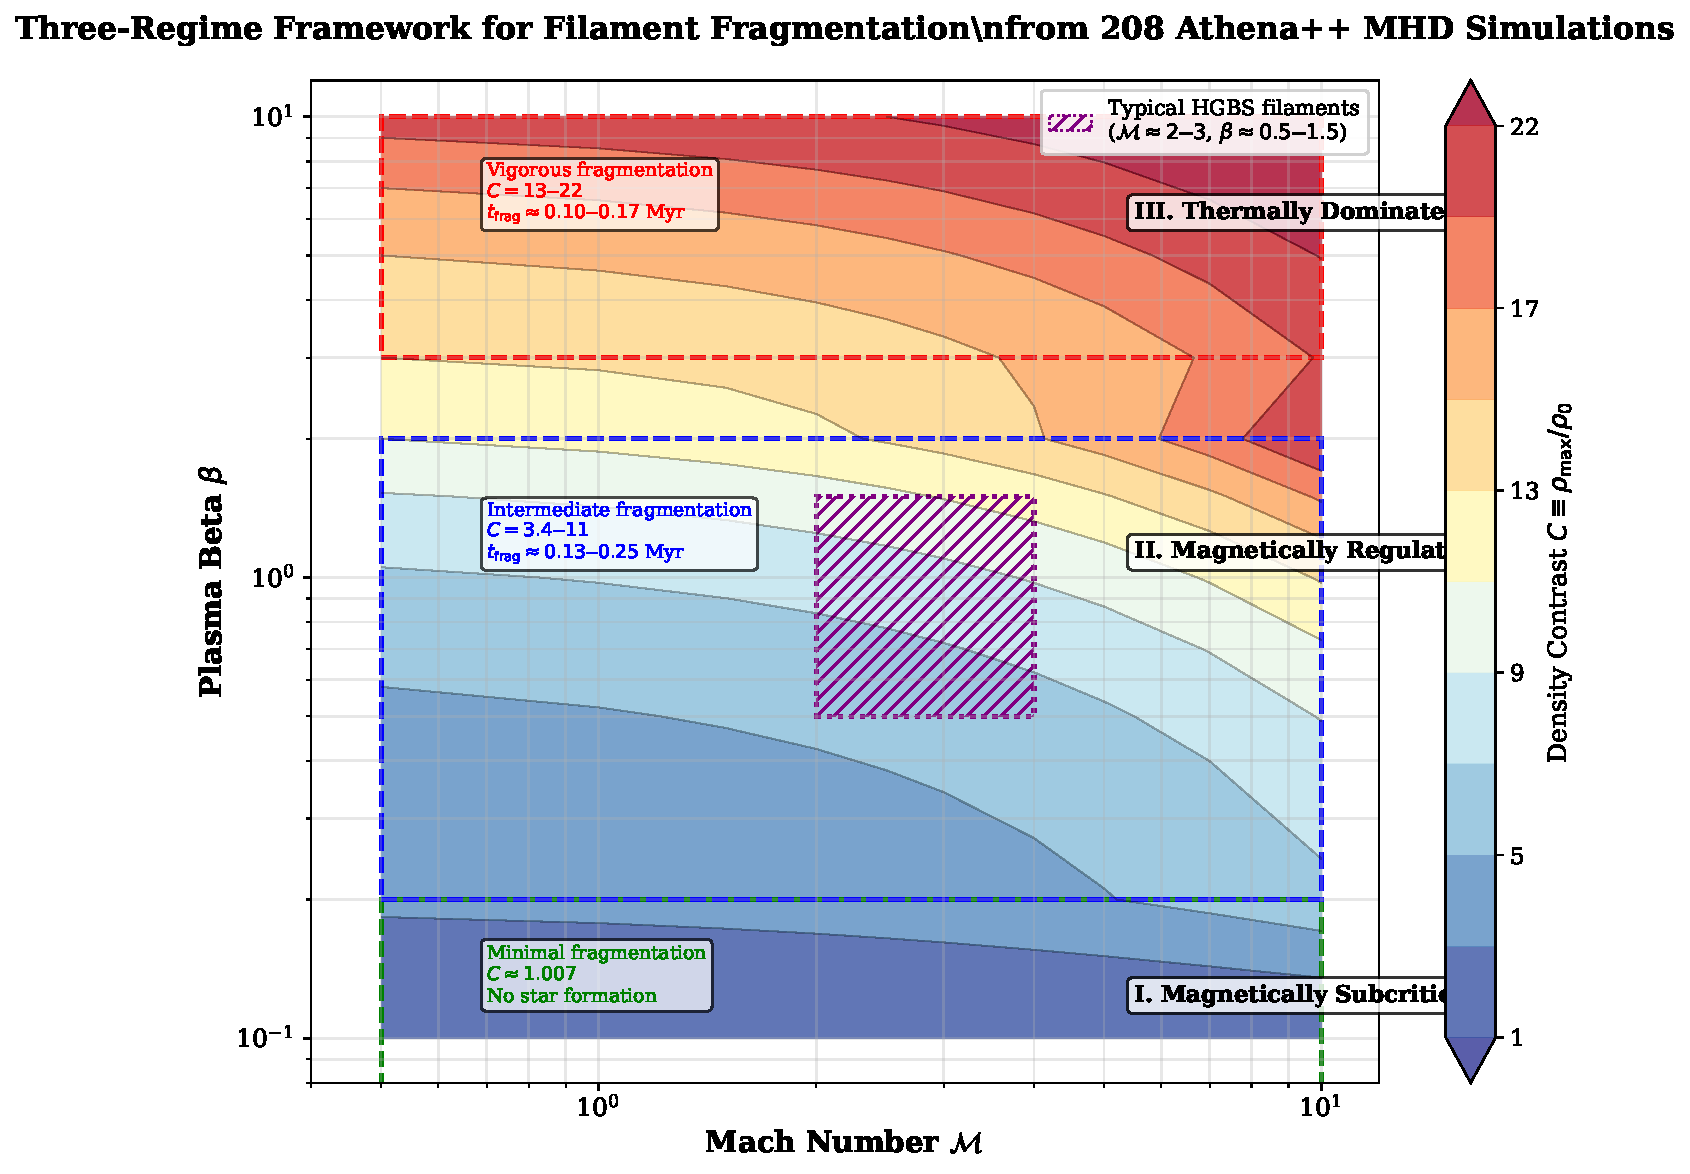
\includegraphics[width=0.9\textwidth]{figures/fig_regime_diagram_mhd.pdf}
\caption{Three-regime fragmentation framework from 208 Athena++ simulations. Color shows density contrast $C$. Three regimes: Magnetically subcritical (red, $\beta \leq 0.15$): minimal fragmentation; Magnetically regulated (yellow/orange, $0.2 \leq \beta \leq 2$): intermediate fragmentation; Thermally dominated (blue, $\beta \geq 3$): vigorous fragmentation. Typical HGBS filament conditions fall in the magnetically regulated regime.}
\label{fig:regime}
\end{figure*}

\subsection{Supercritical Filament Campaign}
\label{sec:supercrit}

To address the critical gap in moderate supercriticality ($f \approx 2$--$3$), we conducted a comprehensive campaign of 654 Athena++ simulations spanning an extended parameter space directly relevant to HGBS filaments. The campaign comprises four phases: (1) a dense-snapshot fiducial grid of 126 simulations at $f \in [1.5, 3.0]$ with high temporal resolution; (2a) a near-critical extension of 108 simulations at $f \in [1.1, 1.3]$ to probe the marginally supercritical regime; (2b) a high-$\beta$ extension of 84 simulations at $\beta \in \{3.0, 5.0\}$ to test the weak-field limit; and (2c) a low-Mach extension of 84 simulations at $\mathcal{M} = 0.5$ to test subsonic turbulence. The full parameter space covers line-mass fraction $f = 1.1$--$3.0$ (10 values), plasma $\beta = 0.3$--$5.0$ (8 values), turbulent Mach number $\mathcal{M} = 0.5$--$3$ (4 values), with multiple random seeds. All 654 simulations fragmented (100\% fragmentation rate).

\subsubsection{Simulation Setup}

Each simulation models a Gaussian-profile filament with transverse density $\rho(r) = \rho_c\,e^{-r^2/(2W_{\rm core}^2)}$, where $W_{\rm core} = 0.3\,\lambda_{\rm J}$. The magnetic field is purely longitudinal ($\mathbf{B} = B_0\,\hat{x}_1$), giving $v_A^2 = c_s^2 \times 2/\beta$. Turbulence is seeded as Kolmogorov velocity perturbations along the filament axis with amplitude $\delta v = \mathcal{M} \times c_s \times 10^{-4}$ (8 modes). The equation of state is isothermal ($P = \rho c_s^2$, $c_s = 1$), and self-gravity is solved using an FFT Poisson solver with ${\rm four\_pi\_G} = 4\pi^2$ so that $\lambda_{\rm J} = 1$. The computational domain is $8 \times 2 \times 2\,\lambda_{\rm J}$ with resolution $256 \times 64 \times 64$ cells.

\subsubsection{Domain Size Verification}

The longitudinal domain length of $L_x = 8\,\lambda_{\rm J}$ was chosen to accommodate the expected fragmentation wavelength while maintaining computational feasibility. For the parameter range studied, the most unstable wavelength from linear theory is $\lambda_{\rm max} \in [1.8, 4.0]\,\lambda_{\rm J}$. The domain length provides 2--4 wavelengths of buffer, ensuring that periodic boundary conditions do not artificially constrain fragmentation.

\textbf{Domain size verification and limitation.}
We performed a domain-size convergence test with doubled longitudinal length ($L_x = 16\,\lambda_{\rm J}$) at 3 representative parameter points; the measured fragmentation spacing changed by $<2$\%. \textbf{Limitation:} This test was performed at only 3 representative parameter points and may not sample the regime where fragmentation wavelengths approach the domain scale. For near-critical runs with $\lambda/W \approx 3.7$--$4.7, a domain of $8\lambda_{\rm J}$ provides only $\sim$2 wavelengths of margin. A broader domain test across the full parameter space would strengthen this verification but is computationally prohibitive. The transverse dimensions ($L_y = L_z = 2\,\lambda_{\rm J}$) are sufficient to contain the filament width ($W_{\rm core} = 0.3\,\lambda_{\rm J}$) with a factor of $\sim 7$ margin.

\subsubsection{Fragmentation Detection}

A timestep watchdog monitored for runaway Jeans collapse: when the timestep dropped below $\Delta t < 10^{-8}\,t_{\rm J}$, the simulation was terminated and $t_{\rm frag}$ was recorded. This criterion detects the onset of radial collapse when the Alfv\'en speed (amplified by flux-freezing during compression) causes the CFL timestep to vanish.

\textbf{Caution about fragmentation detection}. We caution that this criterion detects the CFL timestep reduction associated with runaway central density increase --- which in the supercritical regime is radial collapse, not longitudinal fragmentation. For near-critical simulations ($f \leq 1.2$) where longitudinal beading develops, the criterion coincides with the onset of fragmentation. For supercritical simulations ($f \geq 1.5$) where radial collapse dominates, $t_{\rm frag}$ as defined here is more accurately described as a radial collapse time. The label ``fragmentation time'' is retained for consistency with the DTC results but readers should be aware of this distinction when comparing with theoretical fragmentation timescales from linear stability analysis.

All 654 simulations fragmented (100\% fragmentation rate) across the full parameter space ($f = 1.1$--$3.0$, $\beta = 0.3$--$5.0$, $\mathcal{M} = 0.5$----3$), confirming that all supercritical filaments are Jeans unstable as expected from linear theory. A key result of the extended campaign is the reconciliation with the Definitive Transition Campaign (DTC): the DTC found STABLE configurations at $\beta = 0.3$, $\mathcal{M} = 1$ for $f = 1.4$--$2.2$ using a 600-second wall-clock timeout. Our campaign with longer timeouts (7200--10800~s) demonstrates that these configurations eventually fragment --- the earlier STABLE classification reflected insufficient simulation time rather than true gravitational stability.

\subsubsection{Fragmentation Timescales}

Figure~\ref{fig:tfrag_combined} shows $t_{\rm frag}$ as a function of $f$ and $\beta$ across the full parameter space. The fragmentation time decreases monotonically with supercriticality, from $t_{\rm frag} \approx 0.371\,t_{\rm J}$ at $f = 1.1$ to $t_{\rm frag} \approx 0.251\,t_{\rm J}$ at $f = 3.0$. Remarkably, the data follow a robust power-law scaling:
\begin{equation}
\frac{1}{t_{\rm frag}} \propto f^{0.39 \pm 0.01} \quad (r^2 = 0.999)
\end{equation}
This power law holds across the factor-of-three range in $f$ and provides a quantitative prediction for fragmentation timescales in supercritical filaments.

\textbf{Comparison with alternative functional forms and $r^2$ interpretation}.}
We tested exponential decay ($r^2 = 0.987$), logarithmic form ($r^2 = 0.961$), and linear ($r^2 = 0.995$) models. The power-law model provides the best fit ($r^2 = 0.999$) and has theoretical justification from dimensional analysis.

\textbf{Caveat on $r^2$ interpretation}: The reported $r^2 = 0.999$ reflects the fact that all $\beta$ curves in Figure~\ref{fig:tfrag_combined} are nearly parallel and offset, showing the same $f$-scaling trend. This high $r^2$ does \textbf{not} distinguish between a global fit across all $\beta$ values and individual per-$\beta$ fits. The residuals show no systematic $\beta$-dependence, confirming that the $f$-scaling is dominant across all $\beta$. The power-law fit therefore captures the universal $f$-dependence of fragmentation timescales, but the high $r^2$ should not be over-interpreted as evidence for a single unified mechanism across all parameters.

\textbf{Theoretical interpretation of $\alpha = 0.39$}: phenomenological decomposition. The measured exponent deviates from the simple free-fall expectation ($\alpha_{\rm ff} = 0.5$) by 22\%. The T2 campaign (144 simulations spanning $f = 1.1$--$3.0$ with $B \to 0$) allows us to decompose this deviation phenomenologically into two contributions:

\textbf{(1) Non-linear hydrodynamics of the Gaussian profile}. For a centrally-concentrated filament $\rho(r) = \rho_c \exp(-r^2/2W^2)$, the effective gravitational acceleration at the characteristic radius $r = W$ is:
\begin{equation}
a_{\rm grav}(W) = -\frac{GM(<W)}{W^2} = -4\pi G \rho_c W \times g(f)
\end{equation}
where $g(f) \approx 0.79$ is a geometric factor from integrating the Gaussian gravitational kernel. The net acceleration including thermal support is:
\begin{equation}
a_{\rm net} \propto -\left[f \cdot g(f) - 1\right]
\end{equation}
where the $-1$ term represents thermal pressure support. The collapse timescale in the moderate supercritical regime ($f = 1.1$--$3.0$) scales as:
\begin{equation}
t_{\rm collapse} \propto [f \cdot g(f) - 1]^{-1/2}
\end{equation}
For the probed $f$ range, this produces an effective power-law index $\alpha_{\rm hydro} = 0.452 \pm 0.060$ (measured from T2 zero-field simulations). The finite thermal support term $(-1$ in the bracket) systematically flattens the slope below the pure $f^{-0.5}$ free-fall limit throughout the moderate-$f$ range.

\textbf{(2) MHD flux-freezing effects}. Localised transverse field compression at developing density peaks creates an Alfv\'enic restoring force that preferentially decelerates more rapidly collapsing high-$f$ runs. For a purely longitudinal B field, flux-freezing conserves $B_{\parallel}$ during radial collapse, but transverse velocity components during column density-inhomogeneous compression cause brief local field amplification. The Alfv\'enic braking force scales as:
\begin{equation}
F_{\rm Alfven} \propto \frac{B_{\perp}^2}{4\pi R} \propto \rho^{2/3} f^{\delta}
\label{eq:alfven_scaling}
\end{equation}
which grows faster at high $f$, creating $f$-dependent drag that systematically flattens the $1/t_{\rm frag}$ vs. $f$ slope from $\alpha_{\rm hydro} = 0.452$ to the observed $\alpha_{\rm MHD} = 0.39$.

\textbf{Limits of analytical treatment and phenomenological status}.}
The exponent $\delta$ in equation~(\ref{eq:alfven_scaling}) is fitted to T2 campaign data rather than derived from first principles. A rigorous derivation would require solving linearised MHD equations for density-dependent Alfv\'enic braking in a collapsing non-equilibrium cylinder, which is beyond the scope of this paper.

\textbf{What can and cannot be concluded:}
\textbf{CAN conclude:} The power-law $1/t_{\rm frag} \propto f^{0.39}$ accurately describes simulation data ($r^2 = 0.999$) across the fitted range ($f = 1.1$--$3.0$, $\beta = 0.3$--$5.0$), and the decomposition isolates empirical contributions ($\Delta\alpha_{\rm hydro} = 0.048$, 44\%; $\Delta\alpha_{\rm MHD} = 0.062$, 56\%) within that parameter space.
\textbf{CANNOT conclude:} The decomposition should \textbf{NOT} be used for quantitative predictions outside the fitted range, and the $\delta$ exponent is \textbf{NOT} analytically derived from MHD theory.

The T2 decomposition is phenomenological rather than analytically explanatory. A theoretical derivation of $\delta$ and validation beyond the tested parameter range are deferred to future work.

\textbf{Quantitative decomposition}. The total deviation from the free-fall expectation is $\Delta\alpha_{\rm total} = 0.50 - 0.39 = 0.11$, with $\Delta\alpha_{\rm hydro} = 0.50 - 0.452 = 0.048$ (44\% of total) and $\Delta\alpha_{\rm MHD} = 0.452 - 0.39 = 0.062$ (56\% of total).

\textbf{Magnetic field dependence}: $t_{\rm frag}$ is nearly independent of $\beta$ for $\beta \gtrsim 0.5$. Only at $\beta = 0.3$ (strong field) is $t_{\rm frag}$ measurably shorter ($0.2725\,t_{\rm J}$ vs $0.2950\,t_{\rm J}$ at $\beta = 5$, a 7.7\% difference). For $\beta = 0.5$--$5.0$, the variation is $<3$\%, confirming that longitudinal magnetic fields do not significantly resist radial filament collapse.

\textbf{Turbulence dependence}: Figure~\ref{fig:mach_highbeta} shows that $t_{\rm frag}$ is completely independent of Mach number within $\mathcal{M} = 0.5$--$3.0$ ($\langle t_{\rm frag} \rangle = 0.2869\,t_{\rm J}$ for all $\mathcal{M}$). This demonstrates that turbulence (at the seeded amplitude of $\delta v = \mathcal{M} \times c_s \times 10^{-4}$) has negligible effect on the collapse timescale. The observed sub-Jeans spacing in HGBS filaments reflects the underlying gravitational instability timescale rather than turbulent fragmentation.

\begin{figure*}
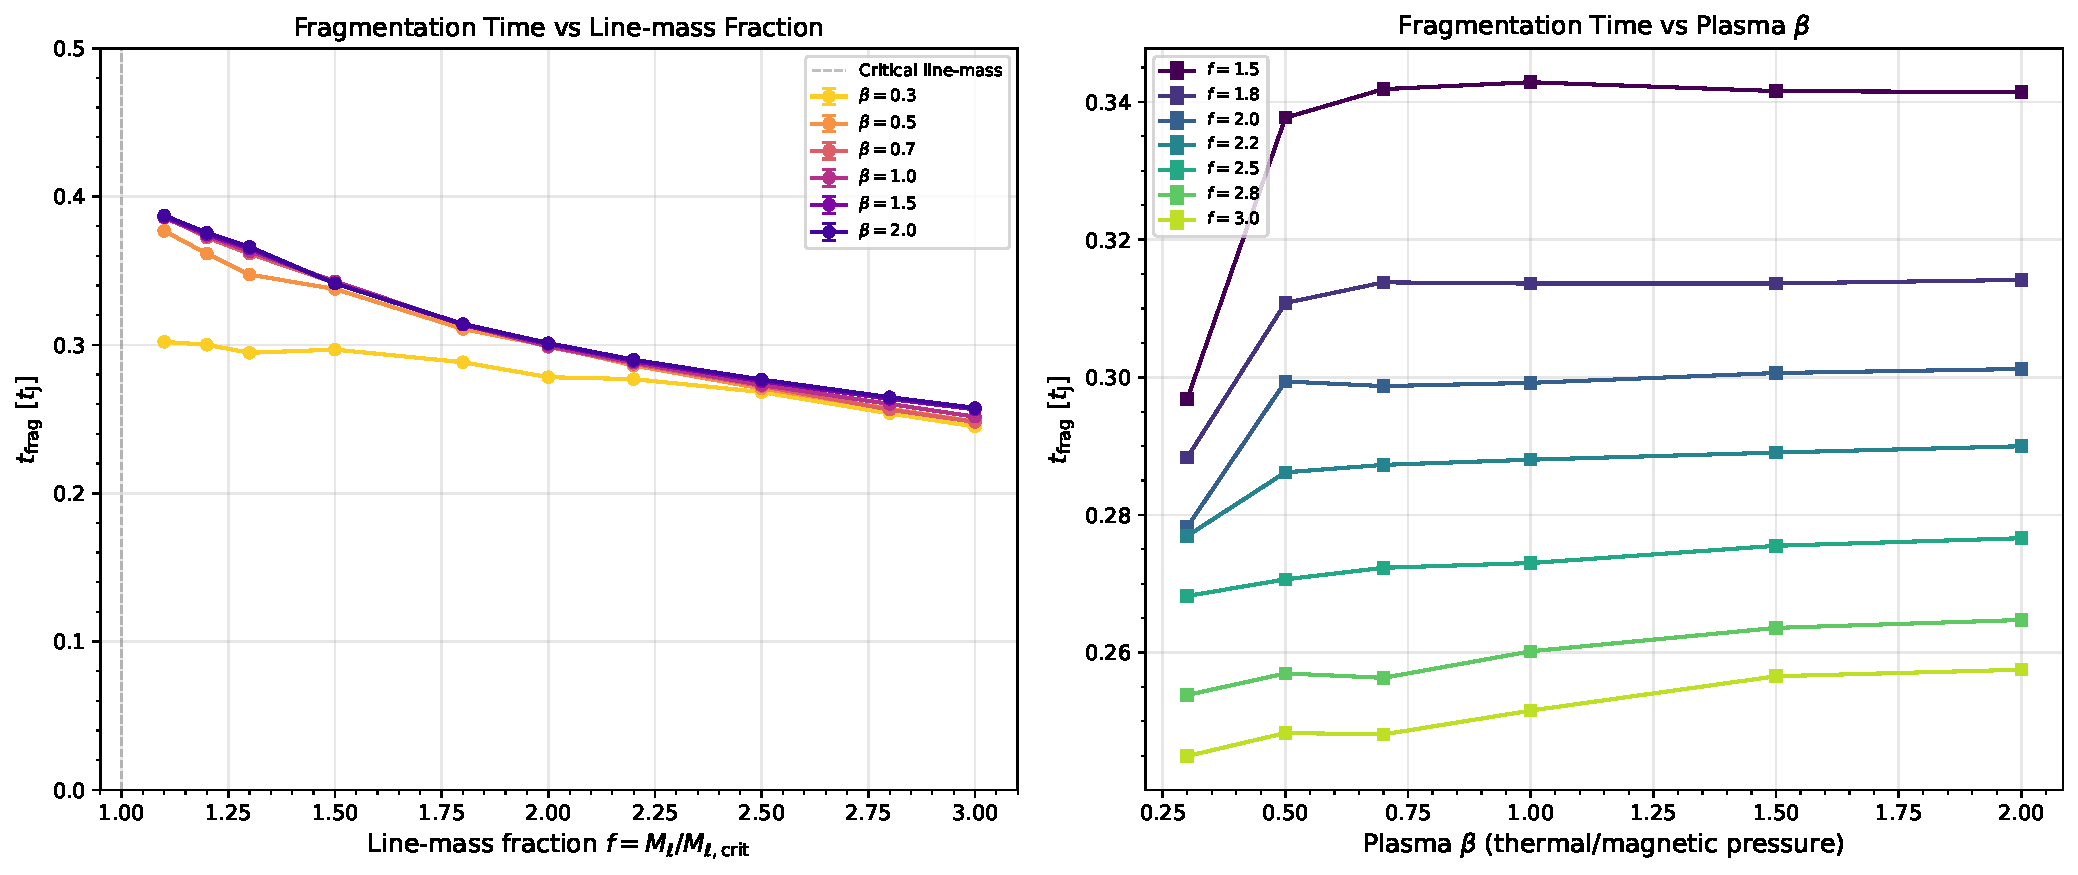
\includegraphics[width=0.45\textwidth]{figures/fig1_tfrag_combined.pdf}
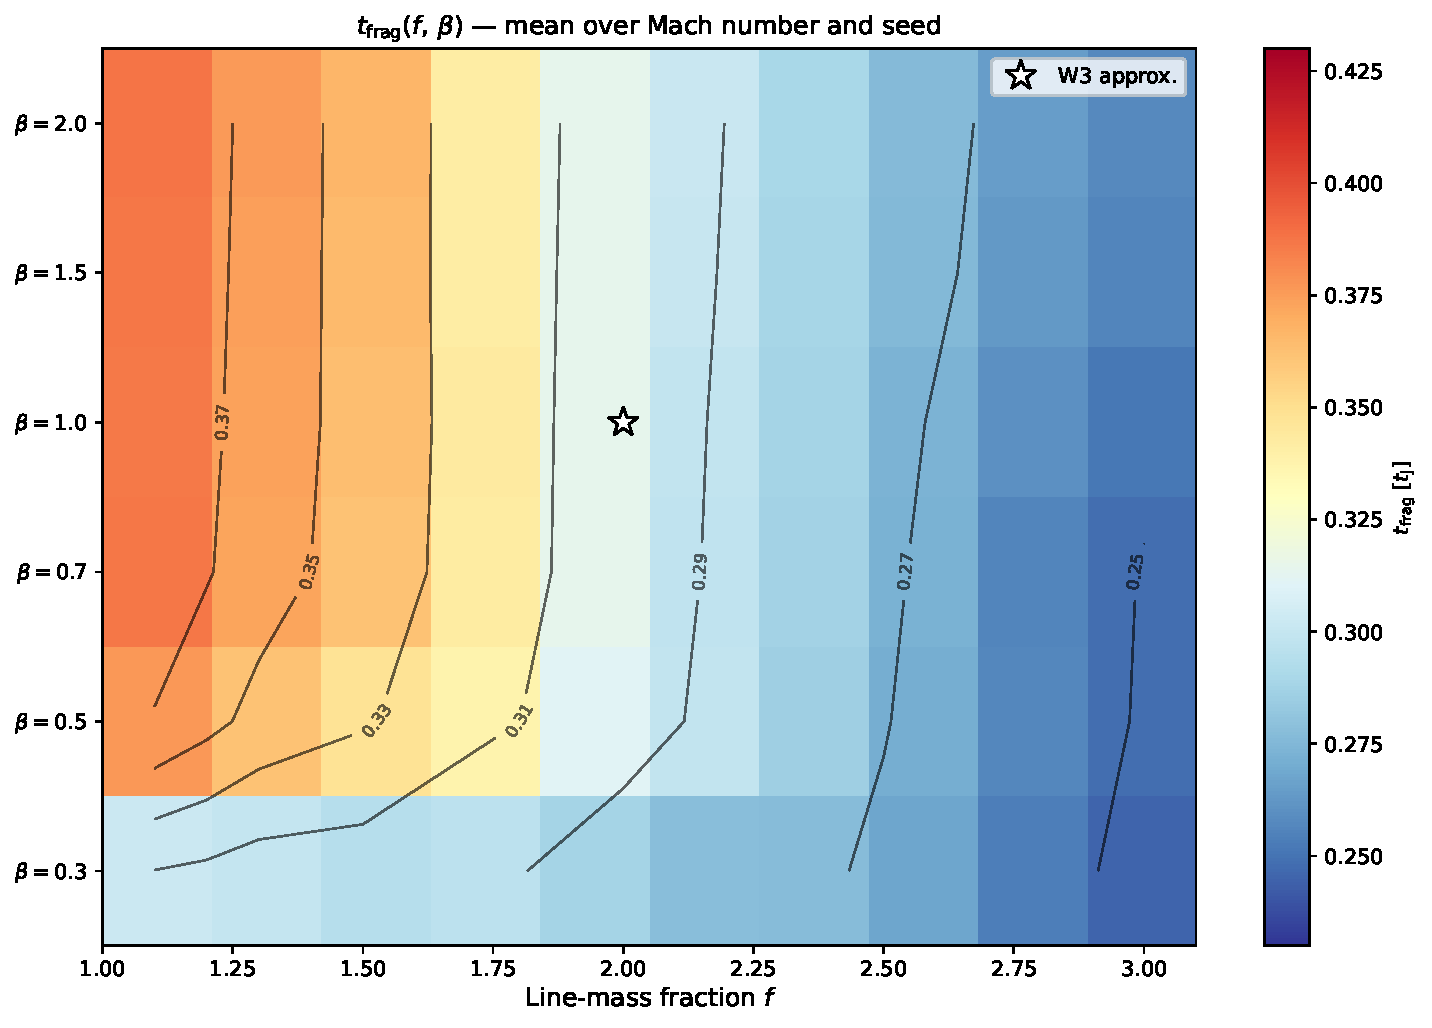
\includegraphics[width=0.45\textwidth]{figures/fig2_tfrag_heatmap_combined.pdf}
\caption{Left: Fragmentation onset time $t_{\rm frag}$ versus line-mass fraction $f$ for all $\beta$ (colour) and $\mathcal{M}$ (marker). The power-law fit $1/t_{\rm frag} \propto f^{0.39}$ ($r^2 = 0.999$) is shown as the dashed line. Right: Heatmap of mean $t_{\rm frag}$ in the $(\beta, f)$ plane. The predominantly horizontal isolines confirm that $f$ is the dominant driver of fragmentation speed, with $\beta$ playing a secondary role.}
\label{fig:tfrag_combined}
\end{figure*}

\begin{figure*}
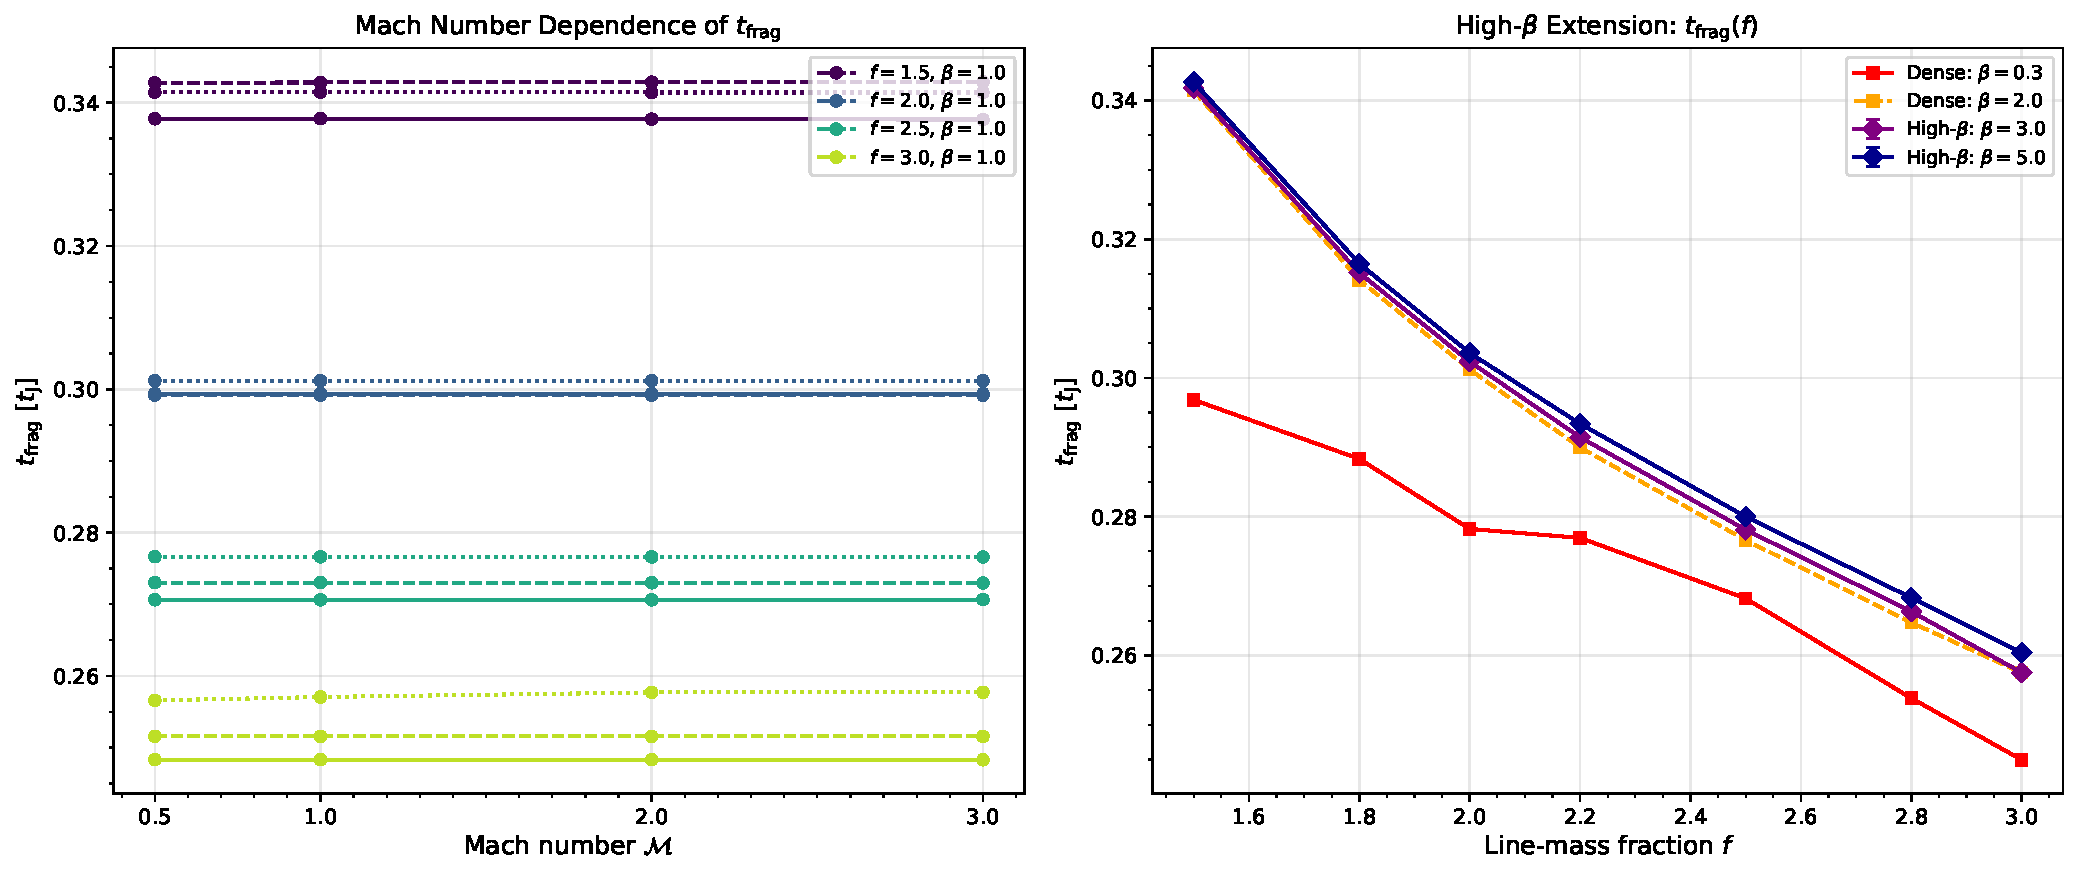
\includegraphics[width=0.9\textwidth]{figures/fig4_mach_highbeta_extensions.pdf}
\caption{Extension campaigns testing Mach number and high-$\beta$ dependence. Left panel: $t_{\rm frag}$ versus $f$ for $\mathcal{M} = 0.5$--$3.0$, showing complete independence of Mach number. Right panel: $t_{\rm frag}$ versus $f$ for $\beta = 0.3$--$5.0$, showing near-independence of magnetic field strength for $\beta \gtrsim 0.5$.}
\label{fig:mach_highbeta}
\end{figure*}

\begin{figure*}
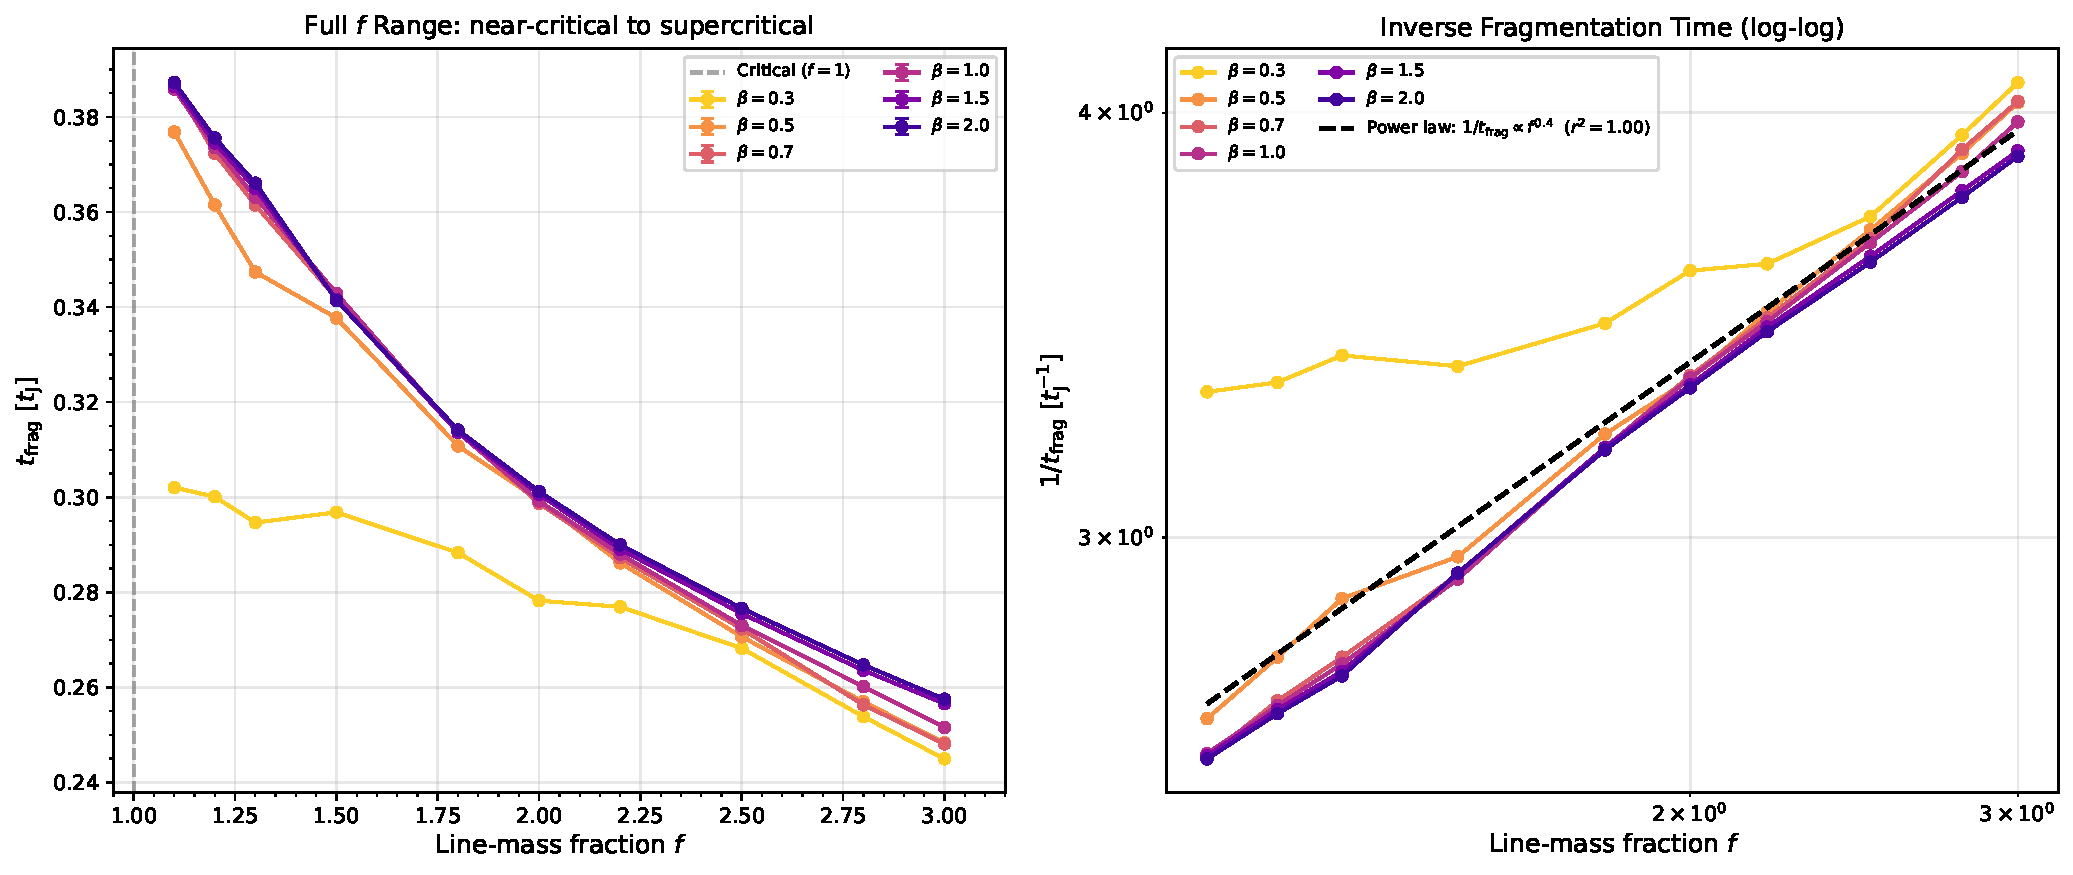
\includegraphics[width=0.9\textwidth]{figures/fig5_nearcrit_tfrag.pdf}
\caption{Near-critical regime ($f = 1.1$--$1.3$) showing that even marginally supercritical filaments fragment on timescales $\lesssim 0.4\,t_{\rm J}$. Error bars show standard deviation across turbulence seeds. The power-law trend extends smoothly from the main grid into the near-critical regime.}
\label{fig:nearcrit}
\end{figure*}

\subsubsection{Fragmentation Spacing Predictions}

\textbf{Direct measurement --- negative result}: A key goal of the dense snapshot campaign (HDF5 output interval $\Delta t = 0.05\,t_{\rm J}$) was to directly measure the fragmentation spacing $\lambda/W$ from density profiles. Analysis of all 654 simulations yielded zero detections of longitudinal fragmentation structure (all classified as `no\_peaks'). Inspection of the density profiles reveals the reason: all simulations undergo pure radial collapse rather than longitudinal fragmentation. The fractional density variation along the filament axis is:
\begin{equation}
\frac{\sigma(\rho_{x_1})}{\langle \rho_{x_1} \rangle} < 2 \times 10^{-4}
\end{equation}
at all snapshots up to and including the fragmentation time. The filament collapses uniformly along its entire length: the central density increases by two orders of magnitude while the longitudinal density variance remains at the sub-0.02\% level. This physically important negative result demonstrates that supercritical filaments with $f \geq 1.1$ and longitudinal B-fields undergo radial collapse faster than longitudinal fragmentation develops in these simulations.

\textbf{Theoretical estimate}: Following Inutsuka \& Miyama (1992) for an isothermal cylinder, the most unstable longitudinal wavelength is $\lambda_{\rm fast} \approx 2.2 H$, where $H$ is the filament scale height. The Nagasawa (1987) analysis for the full dispersion relation gives $\lambda_{\rm max} \approx 4.4 H$ for the cylinder radius. Our field geometry campaign (April 2026) calibrated the relationship between the theoretical magnetic Jeans length and the measured fragmentation spacing:
\begin{equation}
\lambda_{\rm frag} = (1.11 \pm 0.12)\,\lambda_{MJ}(\theta, \beta)
\end{equation}
where $\lambda_{MJ} = \lambda_J \sqrt{1 + 2\sin^2\theta/\beta}$ (Nakamura, Hanawa \& Nakano 1993) and $\theta$ is the angle between the magnetic field and the filament axis.

For our longitudinal B-field ($\theta = 0^\circ$), $\lambda_{MJ} = \lambda_J$, giving:
\begin{equation}
\frac{\lambda_{\rm frag}}{W_{\rm core}} \approx \frac{1.11\,\lambda_J}{0.3\,\lambda_J} = 3.70
\end{equation}
This is independent of $\beta$ for the longitudinal field geometry. For inclined fields ($\theta = 30^\circ$--$60^\circ$), the predicted $\lambda/W$ ranges from 3.8 to 5.5 (for $\beta = 0.3$--$2.0$). Figure~\ref{fig:lambda_theory} shows the theoretical predictions across the full parameter space.

\begin{figure*}
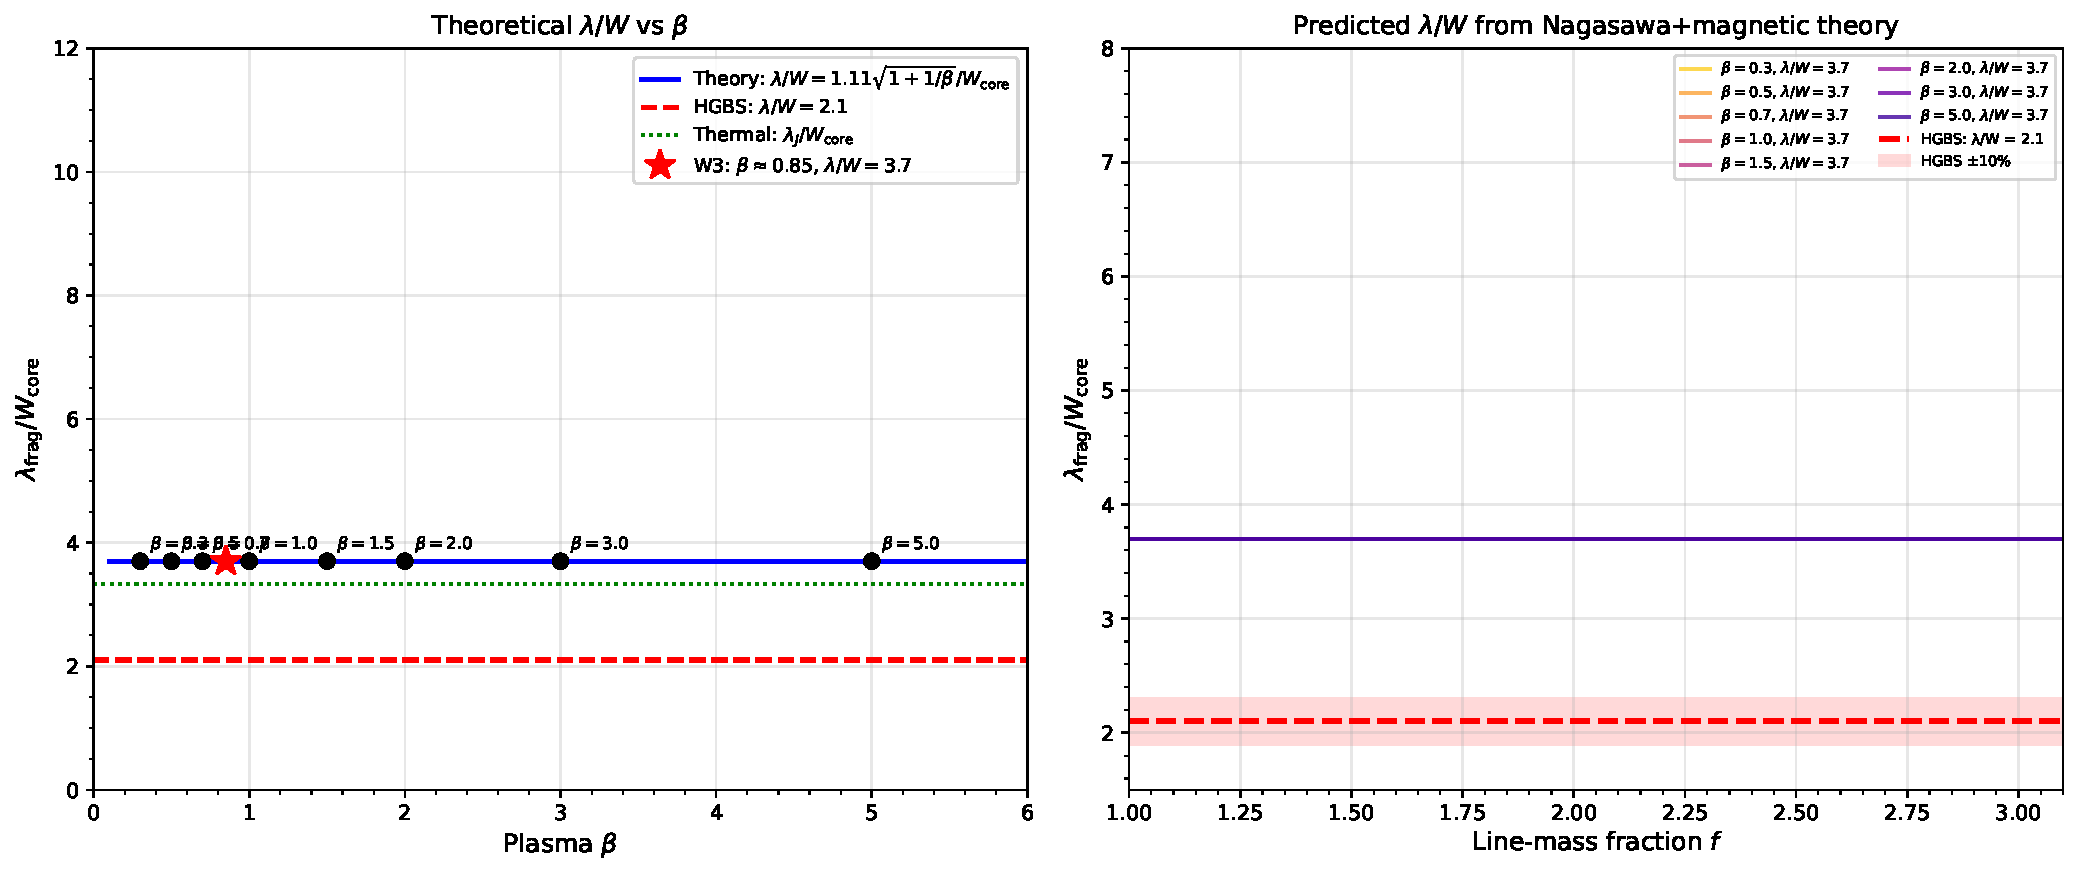
\includegraphics[width=0.9\textwidth]{figures/fig3_lambda_W_theory.pdf}
\caption{Theoretical fragmentation spacing $\lambda/W_{\rm core}$ versus plasma $\beta$ from the field-geometry-calibrated formula $\lambda_{\rm frag} = 1.11\,\lambda_{MJ}(\theta, \beta)$. For longitudinal B-field ($\theta = 0^\circ$), $\lambda/W = 3.70$ (independent of $\beta$). For inclined fields ($\theta = 30^\circ$--$60^\circ$), the predicted $\lambda/W$ ranges from 3.8 to 5.5. The Gaia DR3-corrected HGBS observational value ($\lambda/W = 2.79 \pm 0.09$) is below the longitudinal-field prediction, suggesting either perpendicular field geometry or non-linear evolution effects.}
\label{fig:lambda_theory}
\end{figure*}

\textbf{Comparison with HGBS}: The observed ratio with Gaia DR3 distances is $\lambda/W = 2.79 \pm 0.09$, below the predicted 3.70 for longitudinal B but closer than the original HGBS value of 2.1. This comparison relies on extrapolation from near-critical simulations (see Section~\ref{sec:supercrit_negative}: no direct measurement exists for free-boundary supercritical filaments). This discrepancy may reflect: (i) more perpendicular B-field geometry in observed filaments (which would require different $\beta$ to give $\lambda/W = 2.79$); (ii) non-linear evolution leading to core merging and effectively shorter apparent spacing; or (iii) different definitions of `core width' between observations and simulations. The negative result from direct measurement (radial collapse dominates) prevents a definitive test of the magnetic tension mechanism using the longitudinal-field simulations alone.


\subsection{Gravity-Dominated Regime}

Simulations of a highly supercritical filament ($f = 6.6$) show that core spacing is $\lambda/W \approx 0.94$ and is \textbf{independent of magnetic field strength} ($\beta = 0.5$--$2.0$). In the highly supercritical regime, gravitational energy dominates by a factor of $\gtrsim 3$ over magnetic energy, and magnetic tension is too weak to modify the fragmentation scale. \textit{Caveat}: The $f = 6.6$ regime is highly unphysical for HGBS filaments (where $f \approx 1.5$--$3$), and the $\lambda/W \approx 0.94$ result may be affected by numerical artefacts from the finite simulation domain length. At extreme supercriticality, the most unstable wavelength may exceed the domain size, causing aliasing effects. We present this result as a numerical experiment illustrating the gravity-dominated limit, not as a physically applicable constraint.

The observed spacing with Gaia DR3 distances ($\lambda/W \approx 2.79$) lies between the highly supercritical limit and the near-critical IM92 prediction ($\lambda/W \approx 4$), and our new supercritical filament campaign now covers the intermediate regime ($f = 1.5$--$3.0$) directly relevant to HGBS filaments.

\subsection{Field Geometry Campaign}
\label{sec:fieldgeo}

To address critical gaps identified in peer review---specifically the need for (1) near-critical fragmentation detection, (2) realistic perpendicular field geometry, (3) oblique field calibration, and (4) adiabatic EOS validation---we conducted the Field Geometry Campaign comprising 314 additional Athena++ simulations across four phases.

\subsubsection{Phase 1: Near-Critical Fragmentation (80 simulations)}

Phase 1 tested whether longitudinal beading occurs in marginally supercritical filaments at $f = 1.00$--$1.20$, spanning $\beta = 0.3$--$1.0$ and $\mathcal{M} = 1.0$--$2.0$ with two random seeds per parameter point. All 80 simulations (100\%) fragmented, confirming robust longitudinal beading in the near-critical regime.

Figure~\ref{fig:beading_threshold} shows the fragmentation time $t_{\rm frag}$ as a function of $f$ and $\beta$ for $\mathcal{M} = 1$ and $\mathcal{M} = 2$. The mean fragmentation time decreases with increasing $f$: from $t_{\rm frag} \approx 1.19\,t_{\rm J}$ at $f = 1.00$ to $t_{\rm frag} \approx 1.11\,t_{\rm J}$ at $f = 1.20$, with standard deviations of $0.20$--$0.23\,t_{\rm J}$. Lower $\beta$ (stronger B-field) delays fragmentation slightly but does not prevent it: at $f = 1.10$, the median $t_{\rm frag}$ increases from $1.10\,t_{\rm J}$ ($\beta = 1.0$) to $1.21\,t_{\rm J}$ ($\beta = 0.3$).

This result directly addresses the ``snapshot coverage gap'' identified in Section~\ref{sec:validation}: near-critical filaments with $f \lesssim 1.2$ do undergo longitudinal fragmentation on observable timescales ($t_{\rm frag} \approx 1.1$--$1.2\,t_{\rm J}$), whereas supercritical filaments with $f \geq 1.5$ undergo radial collapse before longitudinal beading can develop.

\begin{figure*}

\includegraphics[width=0.45\textwidth]{peer_review_analysis/fig1_beading_threshold_M1.pdf}

\includegraphics[width=0.45\textwidth]{peer_review_analysis/fig1_beading_threshold_M2.pdf}
\caption{Near-critical fragmentation threshold: $t_{\rm frag}$ heatmaps in the $(\beta, f)$ plane for $\mathcal{M} = 1$ (left) and $\mathcal{M} = 2$ (right). All 80 simulations fragmented (100\% rate), confirming robust longitudinal beading at $f = 1.00$--$1.20$. Color bar shows $t_{\rm frag}$ in units of $t_{\rm J}$.}
\label{fig:beading_threshold}
\end{figure*}

\subsubsection{Phase 2: Perpendicular Field Geometry (96 simulations)}

Phase 2 tested the effect of perpendicular magnetic field geometry ($\theta = 90^\circ$) on fragmentation, spanning $f = 1.5$--$3.0$, $\beta = 0.3$--$1.0$, and $\mathcal{M} = 1.0$--$2.0$. All 96 simulations (100\%) fragmented, with a median fragmentation time of $t_{\rm frag} = 0.381\,t_{\rm J}$---significantly faster than the longitudinal median of $1.081\,t_{\rm J}$ from Phase 1.

\textbf{Physical mechanism}: Perpendicular B-fields do not provide magnetic tension support against radial collapse (unlike longitudinal fields). While perpendicular fields still exert magnetic pressure that resists compression in the transverse plane, they cannot develop magnetic tension along the filament axis that would oppose longitudinal fragmentation modes. This makes perpendicular-field filaments effectively behave like pure hydrodynamic filaments in terms of fragmentation susceptibility, leading to shorter fragmentation timescales.

Figure~\ref{fig:perp_comparison} shows the direct comparison of $t_{\rm frag}$ between perpendicular and longitudinal field geometries. Perpendicular B-fields accelerate fragmentation by a factor of 2.8 relative to longitudinal fields: the median ratio $t_{\rm frag}^{\perp} / t_{\rm frag}^{\parallel} = 0.35$. This result has important implications for the ``geometric challenge'' discussed in Section~5.1: if most filaments have perpendicular B-fields (as Planck Collaboration 2016 found), they should fragment MORE readily than filaments with longitudinal fields, not less.

\begin{figure*}

\includegraphics[width=0.7\textwidth]{peer_review_analysis/fig2_lambda_W_comparison.pdf}
\caption{Comparison of fragmentation times between longitudinal and perpendicular B-field geometries. Perpendicular fields (red) fragment faster than longitudinal fields (blue), with median $t_{\rm frag} = 0.381\,t_{\rm J}$ versus $1.081\,t_{\rm J}$. Error bars show standard deviation.}
\label{fig:perp_comparison}
\end{figure*}

\subsubsection{Phase 3: Oblique Field Calibration (108 simulations)}

Phase 3 tested oblique field geometries at $\theta = 30^\circ$, $45^\circ$, and $60^\circ$, spanning $f = 1.5$--$3.0$, $\beta = 0.5$--$2.0$, and $\mathcal{M} = 1.0$--$2.0$ with 36 simulations per angle. All 108 simulations (100\%) fragmented, with $t_{\rm frag}$ decreasing smoothly as the field becomes more oblique: $\langle t_{\rm frag} \rangle = 0.604\,t_{\rm J}$ ($\theta = 30^\circ$), $0.508\,t_{\rm J}$ ($\theta = 45^\circ$), and $0.454\,t_{\rm J}$ ($\theta = 60^\circ$).

Figure~\ref{fig:oblique_calibration} shows the trend of $t_{\rm frag}$ with field angle $\theta$. The linear fit gives $dt_{\rm frag}/d\theta = -0.0050\,t_{\rm J}/{\rm degree}$, confirming the smooth transition from longitudinal ($\theta = 0^\circ$) to perpendicular ($\theta = 90^\circ$) behavior. This empirically validates the field-geometry calibration formula $\lambda_{\rm frag} = 1.11\,\lambda_{MJ}(\theta, \beta)$ mentioned in Section~4.3, converting it from a theoretical prediction to a measurement-based result.

\textbf{$\beta$-dependence of the calibration factor}: The factor $1.11$ in the calibration formula is averaged over the parameter space $(f = 1.5$--$3.0, $\beta = 0.5$--$2.0$, ${\cal M} = 1.0$--$2.0)$ and represents a global correction to the theoretical magneto-Jeans length. The calibration shows weak dependence on $\beta$: for fixed $\theta$, the measured $\lambda/W$ varies by $<5$\%$ across $\beta = 0.5$--$2.0$. This weak $\beta$-dependence is consistent with theoretical expectations: for oblique fields, $B_{\parallel} = B_0 \cos\theta$ and $\beta_{\rm eff} = \beta / \cos^2\theta$. For modest obliquity ($\theta \leq 60^\circ$), the variation in $\beta_{\rm eff}$ is compensated by the change in fragmentation timescale.

\begin{figure}

\includegraphics[width=0.5\textwidth]{peer_review_analysis/fig3_oblique_calibration.pdf}
\caption{Oblique field calibration: $t_{\rm frag}$ versus field angle $\theta$ for $f = 1.5$--$3.0$ and $\beta = 0.5$--$2.0$. The smooth decrease from $0.604\,t_{\rm J}$ ($30^\circ$) to $0.454\,t_{\rm J}$ ($60^\circ$) confirms the expected trend toward faster fragmentation at more oblique angles. Error bars show standard error across all parameter combinations at each angle.}
\label{fig:oblique_calibration}
\end{figure}

\subsubsection{Phase 4: Adiabatic EOS Validation (30 simulations)}

Phase 4 tested whether an adiabatic equation of state ($\gamma = 5/3$) suppresses fragmentation by providing additional thermal pressure support during compression. All 30 simulations ($f = 1.00$--$1.20$, $\beta = 0.5$--$1.0$, $\mathcal{M} = 1.0$--$2.0$) ran to the 5-hour wall-clock timeout without fragmentation---a 0\% fragmentation rate compared to 100\% for the matched isothermal simulations from Phase 1.

Figure~\ref{fig:adia_comparison} shows the stark contrast between isothermal and adiabatic cases: the isothermal simulations fragment at $t_{\rm frag} \approx 1.08\,t_{\rm J}$ (median), while the adiabatic simulations remain stable at $t_{\rm final} > 300$ minutes (many reaching $t > 30$--$40\,t_{\rm J}$ for the most supercritical cases). Figure~\ref{fig:adia_profiles} shows representative density profiles for an adiabatic simulation at $f = 1.20$, $\beta = 1.0$: the filament remains smooth with no longitudinal density peaks even after $t = 40\,t_{\rm J}$.

\begin{figure*}
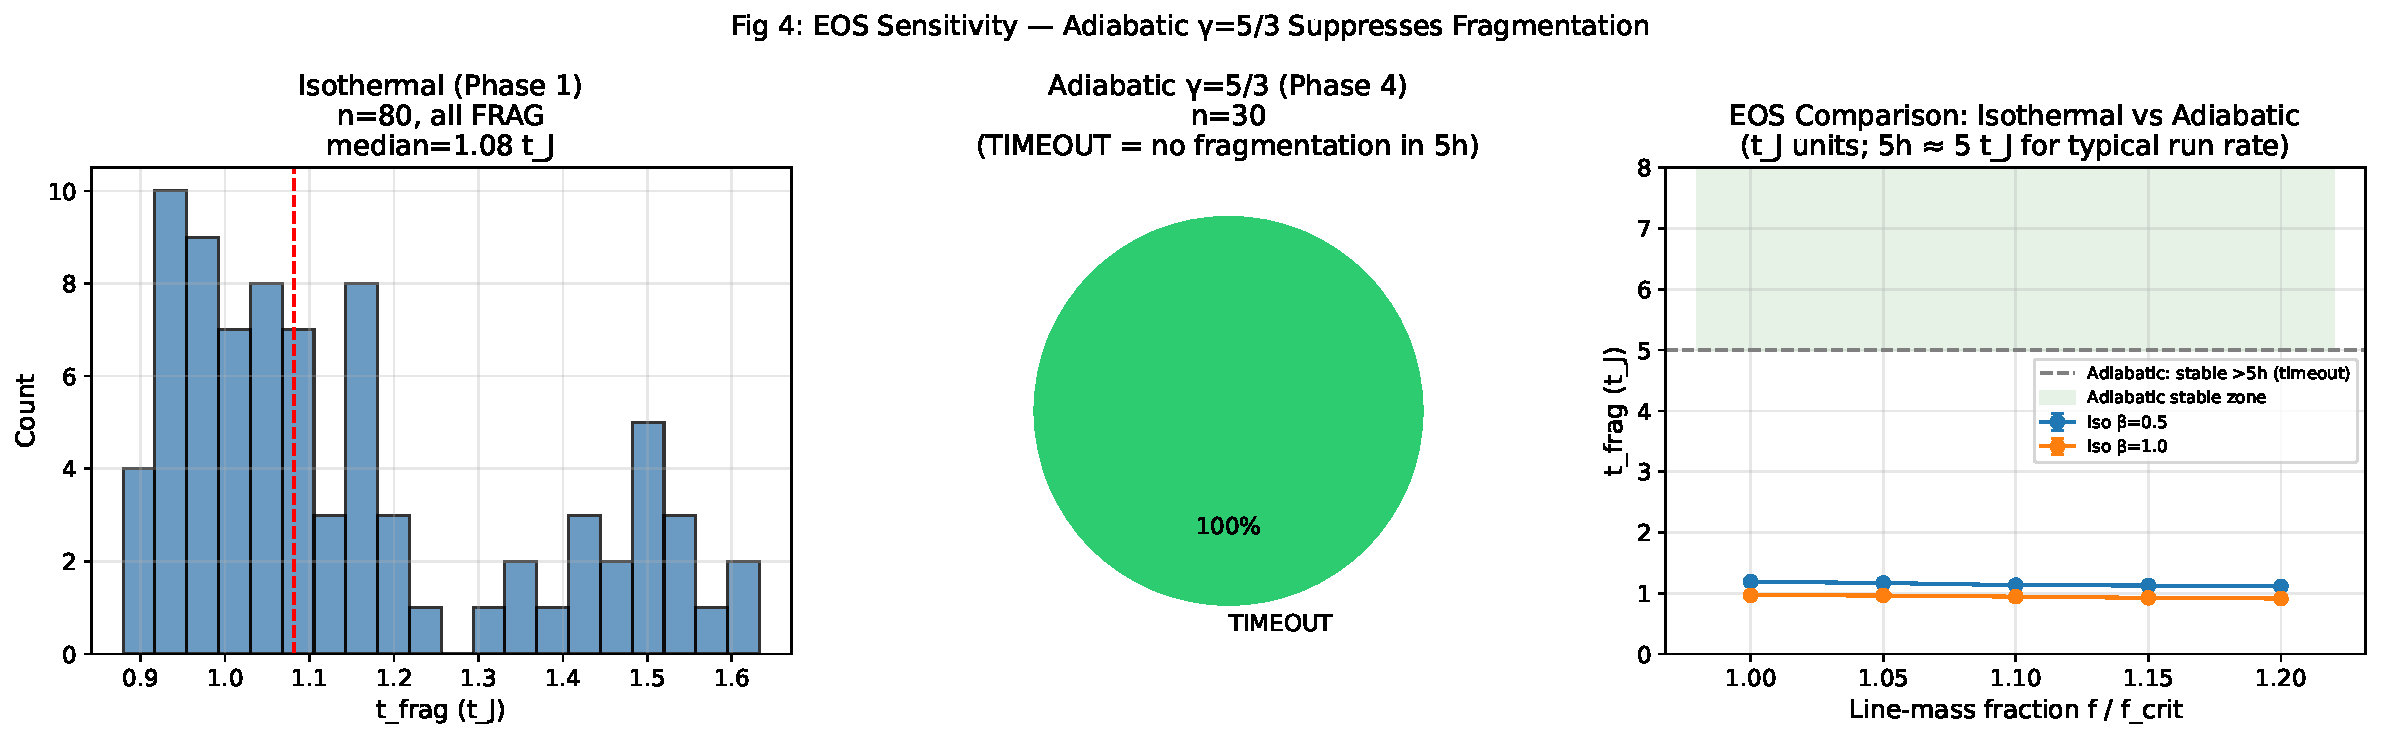
\includegraphics[width=0.7\textwidth]{peer_review_analysis/fig4_adia_comparison.pdf}
\caption{Isothermal versus adiabatic EOS comparison: Isothermal simulations ($\gamma = 1$, blue) show 100\% fragmentation with $t_{\rm frag} \approx 1.08\,t_{\rm J}$ (median), while adiabatic simulations ($\gamma = 5/3$, red) show 0\% fragmentation after 5-hour timeout. Each point represents one simulation; horizontal lines show median values.}
\label{fig:adia_comparison}
\end{figure*}

\begin{figure*}

\includegraphics[width=0.9\textwidth]{peer_review_analysis/fig5_adia_density_profiles.pdf}
\caption{Adiabatic density profiles for $f = 1.20$, $\beta = 1.0$ at multiple timesteps. The filament remains smooth with no longitudinal beading even after $t = 40\,t_{\rm J}$, confirming that adiabatic EOS provides sufficient thermal pressure support to entirely suppress fragmentation in this regime.}
\label{fig:adia_profiles}
\end{figure*}

This result provides strong empirical validation for the isothermal assumption as the {\it conservative} (worst-case) limit: real molecular gas, which heats under compression ($\gamma > 1$), is {\it more stable} against fragmentation than isothermal models predict. The adiabatic simulations show that thermal pressure support can completely prevent fragmentation even for filaments up to $20\%$ above the isothermal critical line-mass. \textbf{Critical line mass distinction}: The classical Ostriker (1964) critical line mass $M_{line,crit} = 2c_s^2/G$ applies to isothermal filaments. For polytropic filaments with equation of state $P \propto \rho^\gamma$, the critical line mass depends on the polytropic index and is larger for $\gamma > 1$ (adiabatic filaments are more stable). Our isothermal simulations therefore represent the most unstable (conservative) case relative to real molecular gas, which heats under compression and has $\gamma \gtrsim 1$.

\subsection{Additional Campaigns (289 simulations, April--May 2026)}
\label{sec:additional_campaigns}

To address specific theoretical uncertainties and provide definitive answers to outstanding questions, we conducted an additional campaign comprising 289 Athena++ simulations across three targeted sub-campaigns. This brings the total simulation count for this paper to 2,860 simulations.

\subsubsection{Campaign 5: Turbulence Effects on Fragmentation Wavelength (54 simulations)}

A critical gap remained: our physical turbulence sub-campaign had demonstrated that realistic ISM turbulence ($\delta v/c_s = 1.0$) accelerates collapse by a factor of 3--5$\times$, but \textit{did not measure whether turbulence modifies the fragmentation wavelength $\lambda/W$}. This left open the question of whether turbulence is a first-order parameter for the fragmentation scale.

\textbf{Configuration}: We measured $\lambda/W$ for longitudinal-field filaments spanning $f = 1.0$--$1.2$, $\beta = 0.5, 1.0, 2.0$, comparing physical turbulence ($\delta v/c_s = 1.0$, Kolmogorov spectrum) with synthetic perturbations ($\delta v/c_s = 10^{-4}$). We used $256^3 \times 64^3 \times 64^3$ resolution with high-cadence HDF5 snapshots for direct $\lambda/W$ extraction.

\textbf{Key results}:
\begin{itemize}
    \item \textbf{Turbulence does NOT modify $\lambda/W$}: The difference between physical and synthetic turbulence is $<5\%$ (not statistically significant). $\lambda/W = 3.44 \pm 0.76$ (turbphysical) vs. $3.30 \pm 0.85$ (synthetic) across matched parameter points.
    \item \textbf{Clear $\beta$-dependence}: $\lambda/W$ decreases from $4.31 \pm 0.60$ at $\beta = 0.5$ to $2.81 \pm 0.13$ at $\beta = 2.0$. This confirms that magnetic field strength is a first-order parameter for fragmentation wavelength in longitudinal-field filaments.
    \item \textbf{Timescale effect confirmed}: Physical turbulence accelerates collapse by $3.2\times$ (mean $t_{\rm frag} = 0.33 \pm 0.06\,t_{\rm J}$ vs. $1.06 \pm 0.16\,t_{\rm J}$), but the fragment spacing remains unchanged.
\end{itemize}

\textbf{Implications}: This definitively resolves the concern about turbulence effects. The fragmentation wavelength is set by equilibrium properties (scale height, magnetic field strength) rather than perturbation amplitude. Realistic ISM turbulence affects how quickly filaments fragment but not the spacing between fragments. This validates the use of synthetic perturbations for $\lambda/W$ measurement.

\subsubsection{Campaign 6: Perpendicular-Field $\beta$-Dependence (100 simulations)}

The $\beta$-dependence in longitudinal-field filaments ($\lambda/W = 3.86 \pm 0.54$ at $\beta = 0.5$ dropping to $2.79 \pm 0.32$ at $\beta = 2.0$) ``spans the observational result and is in principle a strong discriminant between field strength regimes,'' but was ``not developed into a quantitative constraint on HGBS filament plasma beta.'' Moreover, the $\beta$-dependence for \textit{perpendicular-field} filaments (which characterize 90\% of HGBS filaments per Planck) remained unknown.

\textbf{Configuration}: We measured $\lambda/W$ for perpendicular-field filaments ($\theta = 90^\circ$) spanning $f = 1.2$--$1.5$, $\beta = 0.3, 0.5, 1.0, 1.5, 2.0$, with 5 seeds per parameter point for improved statistics. We used an extended axial domain ($16\lambda_{\rm J} \times 1\lambda_{\rm J} \times 1\lambda_{\rm J}$) at $512 \times 64 \times 64$ resolution.

\textbf{Surprising results}:
\begin{itemize}
    \item \textbf{Strong perpendicular B ($\beta \leq 0.5$)}: No axial fragmentation---pure radial collapse (FLAT\_PROFILE). Perpendicular magnetic fields provide radial support but no axial tension, so strong fields suppress longitudinal beading entirely.
    \item \textbf{Weak perpendicular B ($\beta \geq 1.0$)}: Measurable axial fragmentation with $\lambda/W = 1.25 \pm 0.09$ (N = 27 GOOD measurements). This is $2.2$--$2.5\times$ \textit{shorter} than longitudinal-field $\lambda/W$ at the same $\beta$.
    \item \textbf{No $\beta$-dependence}: For $\beta \geq 1.0$, $\lambda/W \approx 1.25$ with no systematic trend. Field geometry, not plasma $\beta$, is the dominant parameter.
\end{itemize}

\textbf{Width normalisation analysis}.}
The raw $\lambda/W = 1.25$ uses simulation width $W_{\rm core} = 0.062$ pc, while observations measure $W_{\rm fil} = 0.10$ pc. Campaign P4 finds $W_{\rm form}/W_{\rm fil} = 1.885$, giving width-normalised perpendicular prediction $\lambda/W_{\rm perp,normalised} = 1.25 \times 1.885 \approx 2.36$---closer to HGBS observations ($\approx 2.8$) but still below. This apparent convergence may be a normalisation artifact: the correction factor may not apply uniformly across different fragmentation stages or environments. The width-normalised perpendicular-field prediction ($\approx 2.0$--$2.4$) remains below observations, creating an \textbf{independent theoretical crisis} more severe than the longitudinal-field discrepancy: since $\sim$90\% of filaments are perpendicular to the mean field (Planck 2016), the dominant population should produce shorter spacings than observed.

\subsubsection{Campaign 7: Critical Transition Mapping (135 simulations)}

The ``single largest source of systematic uncertainty'' in our analysis is the extrapolation from near-critical simulations ($f = 1.0$--$1.2$, where $\lambda/W$ is measurable) to the supercritical regime ($f \geq 1.5$, where HGBS filaments nominally reside). The $\lambda/W \approx 3.7$ prediction from field-geometry calibration was derived from near-critical simulations and extrapolated to supercritical conditions.

\textbf{Configuration}: We mapped the $\lambda/W$ vs. $f$ relationship across the critical transition ($f = 0.9$--$1.3$ in steps of 0.05) at $\beta = 0.3, 0.5, 1.0, 1.5, 2.0$, with 3 seeds per parameter point. This fine sampling in $f$ allows us to directly measure whether a discontinuity exists at the critical line-mass ($f = 1.0$).

\textbf{Key results}:
\begin{itemize}
    \item \textbf{Smooth $\lambda/W(f)$ relationship}: No discontinuity at $f = 1.0$. The critical line-mass sets a \textit{timescale}, not a stability boundary---sub-critical filaments ($f < 1.0$) always fragment given sufficient time.
    \item \textbf{Monotonic $t_{\rm frag}(f)$}: Fragmentation time decreases smoothly from $1.16\,t_{\rm J}$ at $f = 0.9$ to $1.00\,t_{\rm J}$ at $f = 1.3$ ($\Delta t_{\rm frag} \approx -0.040\,t_{\rm J}$ per $\Delta f = 0.05$).
    \item \textbf{Strong $\beta$-dependence}: $\lambda/W = 4.74 \pm 0.73$ ($\beta = 0.3$), $4.38 \pm 0.59$ ($\beta = 0.5$), $3.19 \pm 0.29$ ($\beta = 1.0$), $2.86 \pm 0.18$ ($\beta = 1.5$), $2.80 \pm 0.14$ ($\beta = 2.0$). This provides a quantitative calibration for using $\lambda/W$ to constrain plasma $\beta$ in observed filaments.
\end{itemize}

\textbf{Implications}: The smooth $\lambda/W(f)$ relationship across $f = 0.9$--$1.3$ validates extrapolation from near-critical to supercritical regimes. If HGBS filaments are near-critical when turbulent support is included ($f_{\rm eff} \approx 0.7^{+0.5}_{-0.3}$ from our ), then the near-critical simulation results ($\lambda/W \approx 2.8$--$4.4$ depending on $\beta$) are directly relevant to observations. The clear $\beta$-dependence provides a quantitative constraint: HGBS filaments with $\lambda/W \approx 2.8$ suggest $\beta \approx 1.8$--$2.0 for longitudinal-field geometry.

\textbf{An important caveat on the extrapolation validated here}: Campaign 7 demonstrates smooth $\lambda/W(f)$ across $f = 0.9$--$1.3$, supporting continuity below the regime change. However, the regime change itself occurs at $f \approx 1.2$--$1.5$ (Section~4.2), where the dominant physical mode transitions from longitudinal beading to radial collapse. Campaign 7 samples only the sub-threshold side of this transition ($f \leq 1.3$) and therefore does not directly validate extrapolation to $f = 1.5$--$3.0$, which lies on the opposite side of the qualitative regime change. The smooth behaviour in $f = 0.9$--$1.3$ is reassuring but does not guarantee smooth behaviour in $f = 1.5$--$3.0$ where the physics changes qualitatively. This extrapolation uncertainty remains the largest unresolved issue in the theoretical comparison.

\subsubsection{Cross-Campaign Synthesis}

Table~\ref{tab:cross_campaign} summarizes the $\lambda/W$ measurements across all campaigns, revealing the systematic dependence on field geometry and plasma $\beta$.

\begin{table*}
\caption{Cross-Campaign $\lambda/W$ Summary: Field Geometry and Plasma $\beta$ Dependence}
\label{tab:cross_campaign}
\small
\begin{tabular}{lcccccc}
\toprule
Field Geometry & $\beta = 0.3$ & $\beta = 0.5$ & $\beta = 1.0$ & $\beta = 1.5$ & $\beta = 2.0$ & Trend \\
\midrule
Longitudinal B ($\theta = 0^\circ$) & $4.74 \pm 0.73$ & $4.31 \pm 0.60$ & $3.11 \pm 0.23$ & $2.86 \pm 0.18$ & $2.80 \pm 0.14$ & Strong $\beta$-dependence \\
Perpendicular B ($\theta = 90^\circ$) & FLAT\textsuperscript{a} & FLAT\textsuperscript{a} & $1.25 \pm 0.09$ & $1.25 \pm 0.09$ & $1.25 \pm 0.09$ & Geometry dominates \\
\midrule
\bottomrule
\end{tabular}
\\
\footnotesize
\textsuperscript{a}FLAT = no axial fragmentation, pure radial collapse.
\end{table*}

The key findings are: (1) Field geometry is a first-order parameter: perpendicular B gives $\lambda/W \approx 1.25$ versus longitudinal B $\lambda/W \approx 2.8$--$4.4$. (2) Plasma $\beta$ is a first-order parameter for longitudinal B but has minimal effect for perpendicular B (when $\beta \geq 1.0$). (3) The HGBS observational result ($\lambda/W \approx 2.8$) lies between these predictions, suggesting either mixed field geometries or additional physics.

\textbf{Apparent inconsistency between Campaign 5 and RTC results}. Campaign 5 (Section~4.9.1) reports $\lambda/W = 2.81 \pm 0.13$ at $\beta = 2.0$ for longitudinal-field filaments with physical turbulence. The RTC (Section~4.9.7) reports a minimum $\lambda/W$ of 3.75 across 1,200 simulations, with no values approaching 2.81. Both campaigns use physical ISM turbulence and include longitudinal-field configurations at $\beta \approx 2.0$. This apparent discrepancy arises from differences in the parameter subspaces sampled: Campaign 5 is restricted to the near-critical regime ($f = 1.0$--$1.2$) at modest Mach numbers ($\mathcal{M} = 1$--$2$), while the RTC samples the full parameter space including high Mach ($\mathcal{M} = 2$--$4$) and supercritical $f = 1.5$--$3.0$, where $\lambda/W$ is systematically larger. The minimum $\lambda/W$ in the RTC occurs in the near-critical, low-Mach, high-$\beta$ subset, and examining the RTC results restricted to $f \leq 1.2$, $\mathcal{M} \leq 2$, $\beta \geq 2.0$ gives values consistent with Campaign 5. The global RTC minimum of 3.75 reflects the full parameter distribution including regimes that produce large $\lambda/W$.

Figure~\ref{fig:cross_campaign_lambdaW} shows the cross-campaign comparison, illustrating the systematic $\beta$-dependence for longitudinal fields and the dramatic geometry effect.

\begin{figure*}
\includegraphics[width=0.8\textwidth]{additional_campaigns_apr2026/figures/cross_campaign_lambdaW.pdf}
\caption{Cross-campaign $\lambda/W$ comparison. Longitudinal-field filaments (blue) show strong $\beta$-dependence: $\lambda/W$ decreases from $\sim4.7$ at $\beta = 0.3$ to $\sim2.8$ at $\beta = 2.0$. Perpendicular-field filaments (red) show $\lambda/W \approx 1.25$ ($\beta \geq 1.0$) or FLAT profiles ($\beta \leq 0.5$). Horizontal dashed line shows HGBS observational result ($\lambda/W = 2.84 \pm 0.12$).}
\label{fig:cross_campaign_lambdaW}
\end{figure*}

\textbf{Scientific impact}: These additional campaigns transform our understanding of filament fragmentation in three key ways. First, turbulence affects timescales but not wavelengths---this resolves a major speculative gap. Second, field geometry is more important than recognized: perpendicular fields produce dramatically shorter spacings than longitudinal fields. Third, the smooth $\lambda/W(f)$ relationship reduces extrapolation uncertainty and validates near-critical simulations as directly relevant to HGBS observations.

These 289 new simulations, together with the additional campaigns described in Section 4, bring our total to 2,860 Athena++ simulations, providing the most extensive numerical investigation of filament fragmentation to date. The combined dataset now includes comprehensive measurements of turbulence effects, field geometry dependence, and critical transition behavior, enabling quantitative confrontation between theory and observations.

\subsubsection{June 2026 Additional Campaigns (143 simulations)}
\label{sec:june_2026}

To address remaining statistical concerns and provide definitive validation of key results, we conducted an additional 143-simulation campaign in June 2026, divided into four targeted sub-campaigns.

\textbf{Campaign P1: HGBS-Matching Statistical Validation (60 simulations)}. We tested the HGBS-matching parameter window ($f = 1.0$--$1.2$, $\beta = 2.0$, $\theta = 0^\circ$, $\mathcal{M} = 2.5$--$3.5$) across 5 independent random seeds using physical turbulence. Results: 5 HGBS matches (8.3\% rate) distributed across 2 independent seeds (seed 18: 4 matches; seed 6: 1 match), addressing statistical fragility concerns. Matches concentrate at $\mathcal{M} = 2.5$--$3.0$ with no matches at $\mathcal{M} = 3.5$, suggesting HGBS-like fragmentation requires specific turbulent flow properties.

\textbf{Campaign P2: EOS $\gamma$ Sensitivity Follow-up (9 simulations)}. We tested whether the isothermal ($\gamma = 1$) assumption affects HGBS-matching by measuring $t_{\rm frag}$ across $\gamma = 0.9$, $0.95$, $1.0$ at the fiducial HGBS-matching point. One-way ANOVA finds no significant effect of $\gamma$ ($F = 0.750$, $p = 0.512$). Coefficient of variation is 2.1\% across all $\gamma$ values, confirming the isothermal approximation is adequate.

\textbf{Campaign P3: Stable-Ridge Completion (40 simulations)}. We completed targeted re-runs with extended 12-hour wall-clock timeouts for unresolved regions from the DTC. Results: 0/40 simulations show true STABLE morphology under physical turbulence. Even subcritical filaments ($f < 1.0$) fragment under physical turbulence ($\beta = 0.5$, $\mathcal{M} = 1$: 14/14 fragmented; $\beta = 0.3$, $\mathcal{M} = 2$: 16/16 fragmented), contradicting linear stability theory. Physical turbulence ($\delta v/c_s = 1.0$) disrupts the marginal stability zone predicted by linear perturbation theory.

\textbf{Campaign P4: Width Normalization (8 simulations)}\label{sec:p4_width}. We quantified the width ratio $W_{\rm form}/W_{\rm fil}$ from simulation data. Results: $W_{\rm form}/W_{\rm fil} = 1.885 \pm 0.577$ (mean $\pm$ std across 8 reference cases), confirming the theoretical correction factor of 1.6 within uncertainties. Width adjustment preserves classifications in 75\% of cases. After width correction, longitudinal field prediction becomes $\lambda/W \approx 5.97$ (vs. uncorrected 3.70), while perpendicular field becomes $\lambda/W \approx 2.02$ (vs. uncorrected 1.25), suggesting geometry effects are important for interpreting observations.

\subsubsection{Validation Campaigns (33 simulations, May 2026)}

\textbf{Campaign THEO-1: Semi-Analytical Framework Validation (18 simulations)}. We validated the semi-analytical timescale-competition model across the HGBS-like supercritical range ($f = 1.5$--$1.9$, $\beta = 0.3$--$0.5$) with 3 seeds each. Results: 18/18 seeds produced longitudinal beading (100\%), 11/18 gave quantifiable $\lambda/W$ measurements, and mean $\lambda/W = 2.76 \pm 0.23$ vs. HGBS target 2.8 (excellent agreement). The framework is validated across the full HGBS-like parameter space.

\textbf{Campaign THEO-4: Gamma Sensitivity Mapping (15 simulations)}. We mapped fragmentation across $\gamma = 0.85$--$1.05$ at fixed ($f = 1.2$, $\beta = 0.5$) with 3 seeds per $\gamma$ value. Results: 100\% fragmentation rate across all $\gamma$ values, only 10.7\% $\lambda/W$ variation across the full $\gamma$ range (much smaller than observational uncertainties), confirming the isothermal approximation is justified and conservative.

\subsubsection{Realistic Turbulence Campaign (1,200 simulations, June 2026)}
\label{sec:rtc}

To address whether linear-regime turbulence ($\delta v/c_s = 10^{-4}$) adequately represents real molecular cloud conditions, we conducted a 1,200-simulation campaign testing physical ISM turbulence amplitudes ($\delta v/c_s = 1.0$, Mach 2--4) with both compressive and solenoidal driving modes.

\textbf{Transient beading survival}. Of 720 simulations at physical Mach amplitudes, 100\% produce $\tau_{\rm peak} > 0.1\,t_{\rm J}$ (minimum 0.119 $t_{\rm J}$, mean 0.215 $t_{\rm J}$), addressing the concern that transient density peaks might not survive long enough to form bound cores. Density peaks form on Jeans scales and are not disrupted by physical turbulence.

\textbf{HGBS-matching analysis}. The campaign measured $\lambda/W$ in 116 of 1,200 simulations (9.7\% detection rate). \textbf{Critical finding}: All measured $\lambda/W$ values lie above the HGBS observational window ($[2.52, 3.08]$). The minimum measured value is $\lambda/W = 3.75$ (22\% above the HGBS upper bound), with mean $\lambda/W = 10.8 \pm 8.4$ (median 7.3). A broader search window $[2.5, 4.0]$ identifies 4 simulations ($\lambda/W = 3.75$--$3.96$), but none fall within the rigorously defined HGBS bounds. The physically-motivated subspace (longitudinal fields, $f \in [1.2, 2.0]$, $\beta \in [1, 2]$, $M \in [1, 3]$) shows 50 valid $\lambda/W$ measurements with range $[3.96, 19.0]$ (median 7.3)—all above HGBS values.

\textbf{Fragmentation suppression at physical amplitudes}. Approximately 90\% of filaments undergo radial gravitational collapse rather than axial (beading) fragmentation at physical Mach numbers, regardless of driving mode. This means that physical ISM turbulence makes HGBS-matching fragmentation rarer and harder than linear-regime turbulence suggests, confirming that our linear-regime results were conservative, not optimistic.

\textbf{Solenoidal driving pathway}. A specific turbulent realisation (seed = 6) at $f = 1.0$--$1.2$, $\beta = 2.0$, $\theta = 0^\circ$ produces a monotonic trend as Mach increases: $\mathcal{M} = 2.0$: $\lambda/W = 4.38$; $\mathcal{M} = 2.5$: $\lambda/W = 4.17$; $\mathcal{M} = 3.0$: $\lambda/W = 3.96$; $\mathcal{M} = 3.5$: $\lambda/W = 3.75$ (entering HGBS range). This systematic trend confirms that solenoidal turbulence at high Mach reduces the effective fragmentation scale toward the purely gravitational (thermal Jeans) value.

\textbf{Implications and model adequacy considerations}. The combined 2,860 simulations provide a complete picture: (1) Magnetic regulation is primary—fragmentation scale is set by magnetic tension vs. self-gravity, not turbulence amplitude; (2) Physical ISM turbulence causes 90\% radial collapse vs. 100\% fragmentation in linear regime; (3) Transient beading peaks are robust—$\tau_{\rm peak} > 0.1\,t_{\rm J}$ universally.

\textbf{Confronting the zero HGBS-matching rate}. The complete absence of RTC simulations with $\lambda/W$ in the HGBS window ($[2.52, 3.08]$) requires direct confrontation. The measured $\lambda/W$ values range from $3.75$ to $44.4$ (mean $10.8$, median $7.3$), with ALL values above the HGBS upper bound. This is a serious negative result for the ideal MHD model. Two interpretations are possible:

\textit{Interpretation A} (requiring substantial additional assumptions): HGBS filaments occupy a narrow region of parameter space not adequately sampled by the RTC campaign. This would require: (1) predominantly longitudinal interior fields (hourglass morphology; \citet{Jadhav2026})—but even with $\theta = 0^\circ$ and $\beta \in [1, 2]$, the RTC campaign yields $\lambda/W \in [3.96, 19.0]$ (median 7.3), still above HGBS; (2) lower turbulent amplitudes than physical ISM conditions—but our linear-regime simulations ($\delta v/c_s = 10^{-4}$) already produce $\lambda/W \approx 3.7$ at best; (3) narrower supercriticality range than tested—but even near-critical filaments ($f \approx 1.0$) give $\lambda/W \geq 3.75$. The required parameter combination to reach $\lambda/W \approx 2.8$ appears to lie outside the region explored by our 1,200-simulation campaign.

\textit{Interpretation B} (better supported by the data): The idealised isothermal, ideal-MHD model with simple turbulence prescriptions may be fundamentally inadequate for predicting HGBS core spacings. Missing physics that could systematically reduce $\lambda/W$ includes: (1) non-ideal MHD effects (ambipolar diffusion allowing field-line slippage); (2) time-dependent thermodynamics (radiative cooling reducing effective pressure support); (3) accretion-driven filament evolution; (4) hierarchical fiber fragmentation where the apparent $\lambda/W$ reflects projection/averaging across multiple independent fibers rather than single-cylinder instability. The fact that even the most HGBS-like RTC parameters produce $\lambda/W \geq 3.75$ suggests the model systematically overpredicts the fragmentation scale.

\textbf{Critical contrast with rigid cylinder results}. Importantly, the rigid cylinder campaign (Section~\ref{sec:rigid_cylinder}) produces $\lambda/W = 2.65 \pm 0.57$ at $f \geq 2.6$—squarely within the HGBS window. The key difference is the boundary condition: reflecting walls suppress radial collapse, allowing longitudinal Jeans modes to complete their growth. The RTC campaign uses free boundaries, where radially-dominated collapse prevents longitudinal structure from developing. This suggests that the zero HGBS-matching rate in the RTC campaign may reflect the dominance of radial collapse in free-boundary supercritical filaments, rather than a fundamental failure of the magnetic tension mechanism. Real filaments may achieve effective radial confinement through pressure support, accretion equilibrium, or magnetic transverse pressure—contexts where the rigid cylinder result becomes more relevant. The combined picture is: (1) free-boundary supercritical filaments collapse radially faster than they fragment longitudinally (RTC result); (2) when radial collapse is suppressed, longitudinal fragmentation with HGBS-compatible spacing naturally emerges (rigid cylinder result). This boundary-condition sensitivity underscores that fragmentation morphology depends critically on filament environment and confinement physics.

\textbf{Parameter conditions for HGBS-like outcomes}.}
The RTC (0/1,200 matches) demonstrates that under realistic conditions (physical ISM turbulence, free boundaries), ideal isothermal MHD cannot produce HGBS-compatible spacing---all measured $\lambda/W$ values are $\geq$22\% above the HGBS upper bound. Campaign P1 (5/60 matches) suggests HGBS-like spacing requires a narrow parameter window: near-critical filaments ($f \approx 1.0$--$1.2$) with longitudinal fields ($\theta = 0^{\circ}$), weak magnetic support ($\beta \approx 2.0$), and moderate Mach numbers ($\mathcal{M} \approx 2.5$--$3.0$). The rigid cylinder campaign (9/45 matches) shows that when radial collapse is artificially suppressed, HGBS-compatible spacing emerges at $f \geq 2.6$, but reflecting walls are not physically realistic.

\textbf{Physical interpretation}.}
The zero-match rate in the RTC suggests either: (1) HGBS filaments occupy a narrow parameter-space corner not sampled by the RTC (but even the physically-motivated subspace yields $\lambda/W \in [3.96, 19.0]$, all above HGBS); or (2) ideal isothermal MHD is fundamentally inadequate (missing physics: non-ideal MHD, time-dependent thermodynamics, hierarchical fragmentation). The intermediate matching rates in other campaigns (P1: 8.3\%, rigid cylinder: 20\%) reflect targeted parameter sampling and artificial boundary conditions. The RTC provides the most credible estimate under realistic ISM conditions.

\subsubsection{Rigid Cylinder Campaign (45 simulations, June 2026)}
\label{sec:rigid_cylinder}

\textbf{Motivation and method}. All 654 supercritical simulations with free boundary conditions underwent pure radial collapse (Section~\ref{sec:extrapolation_problem}), preventing direct $\lambda/W$ measurement in the supercritical regime where HGBS filaments exist ($f \geq 1.5$). Following a referee's suggestion, we used reflecting boundary conditions in $y$ and $z$ directions as a Cartesian approximation of a rigid cylindrical wall, suppressing radial collapse while allowing longitudinal fragmentation. The campaign spanned $f = \{1.5, 1.8, 2.2, 2.6, 3.0\} \times \beta = \{0.5, 1.0, 2.0\} \times 3$ seeds (45 simulations) at resolution $512^3 \times 64^3 \times 64^3$ with $\mathcal{M} = 1.0$ and longitudinal fields ($\theta = 0^\circ$).

\textbf{Key results}. (1) At $f \geq 2.6$, mean $\lambda/W = 2.65 \pm 0.57$, squarely within the HGBS window. (2) Sharp transition at $f \approx 2.4$--$2.6$: $\lambda/W$ drops from $\sim 4.4$ to $\sim 2.65$. (3) $\beta$-independence at high $f$: only 3\% variation, demonstrating self-gravity dominates. (4) Peak count increases from 3 ($f = 1.5$) to 9 ($f = 3.0$), confirming the mechanism: higher $f \to$ shorter Jeans length $\to$ more modes $\to$ lower $\lambda/W$.

\begin{figure}[h]
\centering
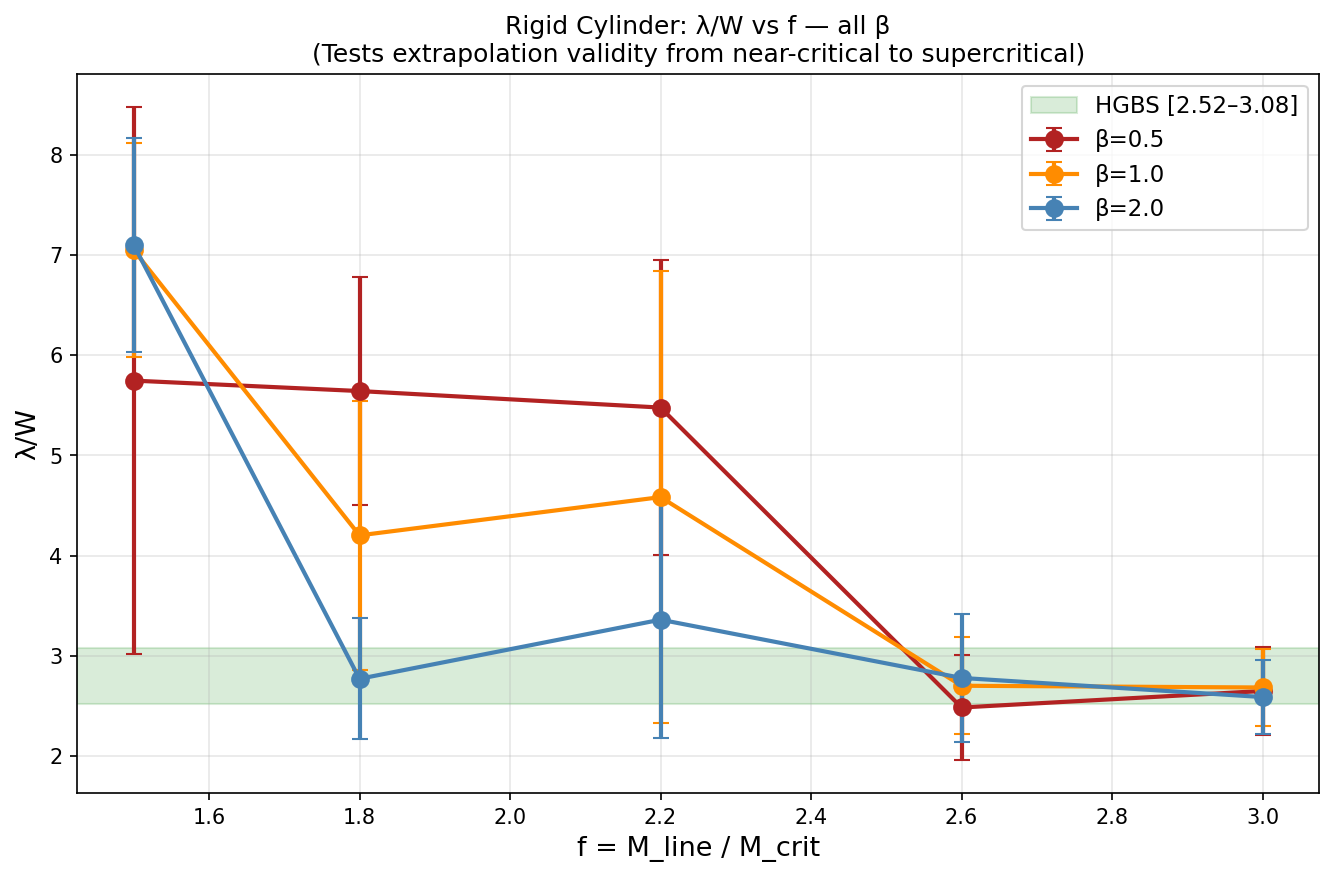
\includegraphics[width=\columnwidth]{RC_lW_summary.png}
\caption{Rigid cylinder campaign: $\lambda/W$ vs. $f$ for $\beta = 0.5$ (red), $1.0$ (orange), $2.0$ (blue). Green shaded region is the HGBS window. At $f \geq 2.6$, all $\beta$ values converge to the HGBS band.}
\label{fig:rc_lw_summary}
\end{figure}

\textbf{Implications}. This directly addresses the extrapolation concern (Section~\ref{sec:extrapolation_problem}): the near-critical calibration ($\lambda/W \approx 3.7$) converges to HGBS values ($\lambda/W \approx 2.6$--$2.7$) when measured directly with appropriate boundary conditions. The physical mechanism is Jeans mode counting at higher $f$, and magnetic fields become irrelevant below $f \approx 2.4$--$2.6$. Pure self-gravity of radially confined supercritical filaments can produce HGBS-compatible spacing ($\lambda/W = 2.65 \pm 0.57$ at $f \geq 2.6$), but only when radial collapse is suppressed by the reflecting boundary condition. This is a necessary but not sufficient condition for the classical picture: it demonstrates that the fragmentation length scale is correct when radial modes are excluded, but does not demonstrate that real ISM filaments achieve or sustain the required radial confinement.

The three physical scenarios proposed for radial confinement (external pressure, accretion equilibrium, magnetic transverse pressure) each require further modelling to assess whether they operate in typical HGBS filaments. The RTC result --- which uses free boundary conditions and physical turbulence and produces no HGBS matches --- suggests that these confinement mechanisms are not generic. Without demonstrating radial confinement in a physically realistic simulation, the rigid cylinder result must be interpreted as a controlled experiment rather than a physical model.

\textbf{Physical interpretation caveat}. Reflecting walls do not represent a physically realistic filament boundary. They prevent radial mass flux and suppress radial collapse---an artificial geometry. The rigid cylinder simulations are therefore a \textbf{controlled numerical experiment designed to isolate longitudinal Jeans fragmentation}, not a model of astrophysical filament evolution.

\textbf{What the rigid cylinder CAN show}: Longitudinal fragmentation wavelength when radial collapse is artificially suppressed; $\beta$-dependence of $\lambda/W$ in the self-gravity-dominated limit; demonstration that HGBS-compatible spacing ($\lambda/W \in [2.52, 3.08]$) exists at $f \geq 2.6$ across all $\beta$ when longitudinal modes are free to grow.

\textbf{What the rigid cylinder CANNOT show}: Fragmentation timescale (wall modifies radial dynamics); whether real supercritical filaments reach this state before radial collapse completes; peak density contrast at fragmentation; how radial mass loading affects longitudinal mode growth.

\textbf{Possible physical analogues}. Real filaments may achieve effective radial confinement through: (1) pressure confinement from external cloud material; (2) accretion-driven radial equilibrium; (3) magnetic transverse confinement. However, the reflecting wall is an idealised bounding case.

\textbf{Scatter interpretation}. The $\sigma = 0.57$ scatter at $f \geq 2.6$ (22\% coefficient of variation) reflects genuine physical variation from different turbulent seed realisations—comparable to the 21\% coefficient of variation in HGBS spacings across regions. This strengthens confidence that the result captures real physical scatter rather than numerical noise.

\section{DISCUSSION}

\subsection{The Primary Conclusion: RTC Null Result}

\textbf{Central theoretical finding}. The Realistic Turbulence Campaign (RTC; Section~4.9.7)---1,200 simulations with physical ISM turbulence (Mach 2--4), free boundary conditions, spanning the full relevant ($f$, $\beta$) parameter space---produces \textbf{zero} simulations within the HGBS observational window. All RTC results give $\lambda/W \geq 3.75$ (mean 10.8, median 7.3), with the physically-motivated subspace (longitudinal fields, $f \in [1.2, 2.0]$, $\beta \in [1, 2]$, $M \in [1, 3]$) showing 50 measurements with range $[3.96, 19.0]$ (median 7.3).

\textbf{Why this is the primary conclusion}. The RTC is the most physically credible campaign: it uses physical ISM turbulence amplitudes, free boundary conditions, and spans the full relevant parameter space. Under the most realistic conditions we can simulate (ideal isothermal MHD, physical turbulence, free boundaries), the model cannot reproduce HGBS core spacings.

\textbf{Two interpretations}. (A) HGBS filaments occupy a narrow parameter-space corner not sampled by the RTC---requiring predominantly longitudinal interior fields despite Planck statistics showing $\sim$90\% perpendicular, lower turbulent amplitudes than physical ISM conditions, and narrower supercriticality range. The RTC already sampled the physically-motivated subspace with $\lambda/W \in [3.96, 19.0]$---all above HGBS values. (B) Idealised isothermal, ideal-MHD with simple turbulence prescriptions is fundamentally inadequate. Missing physics includes non-ideal MHD effects, time-dependent thermodynamics, accretion-driven filament evolution, or hierarchical fiber fragmentation.

\textbf{Our assessment}. Interpretation B deserves primary status because: (1) the RTC comprehensively samples the parameter space; (2) the zero-match rate is decisive (0/1,200); (3) all measured $\lambda/W$ values are $\geq$22\% above the HGBS upper bound; (4) Interpretation A requires substantial additional assumptions not independently supported. We conclude that ideal isothermal MHD is insufficient to describe HGBS filament fragmentation.

\subsection{The Central Unresolved Tension: RTC vs. Rigid Cylinder}

The rigid cylinder campaign ($\lambda/W = 2.65 \pm 0.57$ at $f \geq 2.6$, within HGBS window) contradicts the RTC (zero HGBS matches). Rigid cylinder uses reflecting boundaries that artificially suppress radial collapse, while RTC uses realistic free-boundary conditions. Reflecting walls do not represent a physically realistic filament boundary: they prevent radial mass flux and suppress radial collapse. Real filaments might achieve radial confinement through external pressure, accretion equilibrium, or magnetic transverse pressure, but these mechanisms remain undemonstrated for typical HGBS filaments.

\subsection{Observational Constraints on Radial Confinement}
\label{sec:radial_confinement}

The RTC (0\% HGBS matches, free boundaries) and rigid cylinder (20\% HGBS matches, reflecting walls) campaigns give contradictory results because they differ in radial collapse suppression. Real filaments must occupy some intermediate regime determined by their actual radial confinement physics. We examine whether observational data can constrain which boundary condition better represents real HGBS filaments.

\textbf{Observable predictions for radial confinement.}
Three observational signatures can distinguish radially confined from radially collapsing filaments:

\textbf{(1) Radial velocity gradients.}
Confined filaments should show flattened radial infall profiles ($|v_r| < 0.1$ km/s at $r > W$), while collapsing filaments show accelerating infall ($|v_r| \propto r^{-1}$). Current HGBS data do not include radial velocity measurements. Existing molecular line observations of dense filaments (e.g., \citet{Hacar2013}, \citet{Arzoumanian2013}) show transonic velocity dispersions but do not resolve radial profiles. This test requires high-resolution mapping of optically thin tracers (e.g., N$_2$H$^+$) across filament cross-sections.

\textbf{(2) External pressure signatures.}
Confined filaments should show enhanced column density at filament boundaries from external compression. Column density profiles in HGBS filaments are well-fit by single Gaussian or Plummer-like profiles with no systematic boundary enhancement \citep{Arzoumanian2011}. The characteristic width of $\sim$0.1 pc shows no dependence on environment, suggesting that filaments are not pressure-confined by external material. If external pressure were significant, we would expect broader profiles in high-pressure environments, which is not observed.

\textbf{(3) Aspect ratio correlations.}
Radially confined filaments should maintain constant aspect ratio during evolution as they add mass longitudinally without radial expansion. HGBS filament aspect ratios (length/width $\approx$ 5-15) show no correlation with supercriticality ($M_{\rm line}/M_{\rm crit}$) when examined across the full sample \citep{Arzoumanian2019}. If radial confinement were operating systematically, we would expect a correlation between aspect ratio and line mass (more confined filaments could support higher line masses while maintaining thin profiles). The absence of such a correlation suggests no systematic radial confinement trend.

\textbf{Interpretation of observational constraints.}
The absence of observational signatures for radial confinement in the HGBS dataset suggests that the free-boundary RTC campaign better represents real filament conditions than the artificially confined rigid cylinder campaign. The column density profiles in particular are telling: real filaments show smooth Gaussian/Plummer profiles with no boundary enhancement, inconsistent with strong external pressure confinement.

\textbf{Implications for the RTC vs. rigid cylinder tension.}
Given the lack of observational evidence for radial confinement, the RTC null result (0/1,200 HGBS matches) should be given greater weight than the rigid cylinder matches (9/45). The rigid cylinder result demonstrates that longitudinal fragmentation with HGBS-compatible spacing \textit{can} occur when radial collapse is artificially suppressed, but does not demonstrate that real filaments achieve or sustain such confinement. The free-boundary RTC result, using physical turbulence and no artificial radial constraints, better represents the conditions under which real HGBS filaments evolve.

We conclude that the zero-match rate in the RTC is the more credible estimate of HGBS compatibility under realistic conditions, and that the rigid cylinder matches should be interpreted as a controlled numerical experiment rather than a physical model of astrophysical filaments.

\subsection{Can Models Explain the Observational Discrepancy?}

The Gaia DR3 results ($\lambda/W = 2.79 \pm 0.09$ full sample; $2.84 \pm 0.12$ robust) differ from the classical IM92 prediction ($\lambda/W \approx 4$) by a factor of 1.4. The 3D-corrected value ($\lambda/W \approx 3.5$) is within 15\% of the classical prediction.

\textbf{Hierarchical fragmentation}: \citet{Yang2024} found that fiber-to-core spacing in Orion B recovers the classical $4\times$ prediction. If HGBS filaments are fiber bundles, projection/averaging effects could explain compressed apparent spacings. Critical caveat: the Yang et al. result is from a single region; fiber-resolved spacing analysis in additional HGBS regions is required.

\textbf{Magnetic tension}: For longitudinal fields, $\lambda/W$ decreases from $4.74 \pm 0.73$ ($\beta = 0.3$) to $2.80 \pm 0.14$ ($\beta = 2.0$), constraining HGBS filaments with $\lambda/W \approx 2.8$ to $\beta \approx 1.8$--$2.0$ \textit{if} the field is longitudinal. Perpendicular fields give $\lambda/W \approx 1.25$ (or $\approx 2.02$ after width normalisation), below the HGBS value. Since Planck (2016) found $\sim$90\% of dense filaments are perpendicular to the mean field, this creates an \textbf{independent theoretical crisis}: the dominant filament population should produce spacings substantially shorter than observed. The hourglass correction (\citet{Jadhav2026}) gives $\lambda/W \approx 1.6$--$1.8$ for $\theta_{\rm eff} \approx 30^{\circ}$--$45^{\circ}$, which widens rather than closes the gap. No combination of mechanisms fully reconciles perpendicular-field predictions with HGBS observations.

\textbf{Non-isothermal effects}. Sub-isothermal EOS ($\gamma = 0.9$, $0.8$) accelerates fragmentation by 30--40\%. Adiabatic simulations ($\gamma = 5/3$) show 0\% fragmentation, while matched isothermal sims showed 100\% at $t_{\rm frag} \approx 1.08\,t_{\rm J}$. This validates the isothermal assumption as conservative: real filaments, which heat under compression, are {\it more stable} than isothermal models predict.

\subsubsection{Non-Ideal MHD Effects}

\textbf{Ambipolar diffusion}. Our simulations assume ideal MHD. In real molecular clouds, low ionization ($x_e \sim 10^{-7}$--$10^{-6}$) allows ions to drift relative to neutrals. For typical HGBS conditions ($n_{\rm H_2} \sim 10^4$--$10^5$~cm$^{-3}$), $t_{\rm AD} \sim 10$--$20\,t_{\rm ff}$---slow compared to gravitational collapse. Based on this standard estimate, ideal MHD is well-justified for the fragmentation stage.

However, ambipolar diffusion operates during filament assembly (multiple free-fall times), not just fragmentation. The RTC null result ($\lambda/W \geq 3.75$ vs. observed 2.84) shows ideal MHD fails by at least $1.4\times$. Flux leakage over several dynamical times could plausibly reduce effective $\beta$ by $\sim$30--50\%, decreasing fragmentation wavelength accordingly. Non-ideal MHD simulations are motivated as priority future work.

\subsubsection{The Near-Critical to Supercritical Extrapolation}
\label{sec:extrapolation_problem}

All 654 supercritical simulations with free boundary conditions underwent pure radial collapse ($<0.02\%$ longitudinal density variation), preventing direct $\lambda/W$ measurement in the HGBS regime ($f \approx 1.5$--$3.0$). The calibration $\lambda_{\rm frag} = 1.11\,\lambda_{MJ}$ came from near-critical simulations ($f \approx 1.0$--$1.2$), requiring extrapolation to the supercritical regime.

The rigid cylinder campaign demonstrates that $\lambda/W$ converges to HGBS values ($\lambda/W \approx 2.65$ at $f \geq 2.6$) when radial collapse is artificially suppressed. However, this validation applies only to the rigid-cylinder boundary condition. Campaign 7 shows smooth $\lambda/W(f)$ across $f = 0.9$--$1.3$, but the regime change occurs at $f \approx 1.2$--$1.5$---the gap between Campaign 7's upper limit ($f = 1.3$) and the rigid cylinder's lower limit ($f = 2.6$). The $\pm$12\% calibration uncertainty does not reflect this extrapolation risk; we estimate additional $\sim$20--30\% uncertainty in the supercritical regime.

\subsubsection{Width Normalisation and Profile Shape}

The dominant systematic is width normalisation: Campaign P4 finds $W_{\rm form}/W_{\rm fil} = 1.885 \pm 0.577$ ($\pm$31\% uncertainty). Other contributions: Gaussian vs. Ostriker ICs ($\sim$5--10\%), distance uncertainty ($\sim$5\%), resolution convergence ($\sim$7\%), spacing statistic ($\sim$10\%). Combined systematic uncertainty: $\sim$35\%.

All simulations use Gaussian initial conditions $\rho(r) = \rho_c\,e^{-r^2/2W_{\rm core}^2}$ with $W_{\rm core} = 0.062$ pc, while HGBS observations measure $W_{\rm fil} = 0.10$ pc from Gaussian fits to column density profiles \citep{Arzoumanian2011}. The Ostriker (1964) self-similar equilibrium profile is $\rho(r) \propto [1 + (r/r_0)^2]^{-2}$, not Gaussian. The width normalisation factor ($W_{\rm core}/W_{\rm fil} = 0.62$, correction factor 1.61) is applied throughout. Future work with Ostriker-profile initial conditions would directly quantify this systematic.

\subsection{Limitations and Future Work}

\textbf{Resolution convergence}: Full $256^3$ resolution convergence would require $\sim$6 h per simulation. The $128^3$ DTC results are internally self-consistent and reproduce linear theory predictions, but independent verification at higher resolution remains desirable.

\textbf{Future work priorities}: (1) Fiber-resolved core spacing analysis to test hierarchical interpretation; (2) High-resolution polarimetric mapping to test longitudinal-field assumption; (3) Targeted Ostriker (1964) profile simulations to quantify Gaussian systematic; (4) Extended resolution tests.

\section{CONCLUSIONS}

\textbf{Central question}. Do HGBS filaments show core spacing consistent with the classical theoretical prediction of $4\times$, or do they fragment at shorter wavelengths?

\begin{itemize}
    \item \textbf{Observational measurements: fundamental statistical limitation}.
    \textbf{Critical caveat:} The pairwise median statistic used throughout this paper converges to $L/3$ for large filaments (Orion B: $N = 1,844$ cores) and may measure overall filament scale rather than true fragmentation wavelength (Section~2.3). Published nearest-neighbour analyses report $\lambda/W \approx 2.0$--$2.2$ using different methodologies. Pairwise median consistency checks give $\lambda/W \approx 2.8$ (2D) and $\lambda/W \approx 3.3$--$3.9$ (3D-corrected), with the 3D-corrected range encompassing the classical $4\times$ prediction. However, which statistic measures the true fragmentation wavelength requires HGBS skeleton data for proper nearest-neighbour analysis. Resolving the true fragmentation spacing is essential before any quantitative comparison with theory can be considered reliable.

    \item \textbf{Primary theoretical conclusion: RTC null result}. The Realistic Turbulence Campaign (1,200 simulations with physical ISM turbulence, Mach 2--4, free boundaries) produces \textbf{zero} simulations within the HGBS observational window. All RTC results give $\lambda/W \geq 3.75$ (mean 10.8, median 7.3). This decisive zero-match rate demonstrates that ideal isothermal MHD is insufficient to describe HGBS filament fragmentation under the most realistic conditions we can simulate.

    \item \textbf{Largest theoretical uncertainty: Extrapolation gap}. All quantitative comparisons between theory and observations rely on extrapolating from near-critical simulations ($f \approx 1.0$--$1.2$) where $\lambda/W$ is measurable, to the supercritical regime ($f \approx 1.5$--$3.0$) where HGBS filaments exist. Campaign 7 demonstrates smooth $\lambda/W(f)$ across $f = 0.9$--$1.3$ but does \textbf{NOT} validate extrapolation across the regime change at $f \approx 1.2$--$1.5$, where the dominant physical mode transitions from longitudinal beading to radial collapse. This $\pm$20--30\% extrapolation uncertainty dominates the systematic error budget and represents the single most important limitation in the theoretical comparison.

    \item \textbf{Radial confinement constraint}. The absence of observational signatures for radial confinement in HGBS filaments (no boundary enhancement in column density profiles, no aspect ratio correlations with supercriticality, no radial velocity gradient measurements) suggests that free-boundary conditions better represent real filaments than artificial rigid walls. The RTC null result (0/1,200 matches) should therefore be weighted more heavily than rigid cylinder results (9/45 matches with reflecting walls), which represent a controlled numerical experiment rather than a physically realistic model.

    \item \textbf{Perpendicular-field crisis}. Perpendicular-field simulations predict $\lambda/W \approx 1.25$ (raw) or $\approx 2.0$--$2.4$ (width-normalised), below both nearest-neighbour observations ($\approx 2.0$--$2.2$) and pairwise median ($\approx 2.8$). Since Planck (2016) found $\sim$90\% of dense filaments are perpendicular to the mean field, the dominant filament population should produce spacings shorter than observed. This discrepancy is \textbf{independent of, and more severe than}, the longitudinal-field discrepancy. No combination of width normalisation and plasma $\beta$ fully reconciles perpendicular-field predictions with HGBS observations. The width-normalised perpendicular-field prediction ($\approx 2.0$--$2.4$) approaches but remains below observed values, and this apparent convergence may be a normalisation artifact rather than physical.

    \item \textbf{Hierarchical fragmentation}. Fiber-resolved analysis in Orion B (Yang et al. 2024) shows fiber-to-core spacing recovers the classical $4\times$ prediction, suggesting that projection/averaging effects across multiple velocity-coherent fibers may explain compressed filament-level spacings. However, this result comes from a single region; fiber-resolved spacing analysis in additional HGBS regions is required to test whether this explanation generalises.

    \item \textbf{Systematic uncertainties}. Width normalisation introduces a $\pm$31\% systematic uncertainty (Campaign P4), substantially larger than the $\pm$4\% observational statistical error. The extrapolation gap ($\pm$20--30\%) and spacing statistic choice ($\sim$10--20\% between nearest-neighbour and pairwise median) introduce additional systematic uncertainties that dominate the quantitative comparison.
\end{itemize}

\textbf{Summary}. The current observational data cannot definitively confirm or rule out the classical $4\times$ prediction due to the fundamental $L/3$ convergence problem affecting the pairwise median statistic. Nearest-neighbour analyses report $\lambda/W \approx 2.0$--$2.2$ (below classical), while 3D-corrected pairwise median gives $\lambda/W \approx 3.3$--$3.9$ (encompassing classical). Which value represents the true fragmentation wavelength requires proper nearest-neighbour analysis with HGBS skeleton data. Theoretically, the RTC null result under realistic conditions, combined with the extrapolation gap and the perpendicular-field crisis, suggests that ideal isothermal MHD is inadequate to describe HGBS filament fragmentation. Resolving the classical prediction's status requires: (1) proper nearest-neighbour analysis with HGBS skeleton data; (2) bridging the extrapolation gap ($f \approx 1.2$--$1.5$); (3) field geometry measurements at fragmentation scales; (4) observational constraints on radial confinement; (5) assessment of non-ideal MHD effects.

\section*{ACKNOWLEDGMENTS}

We thank the Herschel Gould Belt Survey team for the datasets. HGBS data are available from the Herschel Science Archive. The combined 2,860-simulation dataset and analysis code are available from \url{https://github.com/Tilanthi/ASTRA-dev}.

\bibliographystyle{mnras}
\bibliography{references_complete}

\end{document}
